%%%%%%%% ICML 2022 EXAMPLE LATEX SUBMISSION FILE %%%%%%%%%%%%%%%%%

\documentclass[nohyperref]{article}

% Recommended, but optional, packages for figures and better typesetting:
\usepackage{microtype}
\usepackage{graphicx}
%\usepackage{subfigure}
\usepackage{booktabs} % for professional tables

% hyperref makes hyperlinks in the resulting PDF.
% If your build breaks (sometimes temporarily if a hyperlink spans a page)
% please comment out the following usepackage line and replace
% \usepackage{icml2022} with \usepackage[nohyperref]{icml2022} above.
\usepackage{hyperref}


% Attempt to make hyperref and algorithmic work together better:
\newcommand{\theHalgorithm}{\arabic{algorithm}}

% Use the following line for the initial blind version submitted for review:
% \usepackage{icml2022}

% If accepted, instead use the following line for the camera-ready submission:
\usepackage[accepted]{icml2022}

% For theorems and such
\usepackage{amsmath}
\usepackage{amssymb}
\usepackage{mathtools}
    \usepackage{amsthm}

% if you use cleveref..
\usepackage[capitalize,noabbrev]{cleveref}


%%%%%%%%%%%%%%%%%%%%%%%%%%%%%%%%
% THEOREMS
%%%%%%%%%%%%%%%%%%%%%%%%%%%%%%%%
\theoremstyle{plain}
\newtheorem{theorem}{Theorem}[section]
\newtheorem{proposition}[theorem]{Proposition}
\newtheorem{lemma}[theorem]{Lemma}
\newtheorem{corollary}[theorem]{Corollary}
\theoremstyle{definition}
\newtheorem{definition}[theorem]{Definition}
\newtheorem{assumption}[theorem]{Assumption}
\theoremstyle{remark}
\newtheorem{remark}[theorem]{Remark}

% Todonotes is useful during development; simply uncomment the next line
%    and comment out the line below the next line to turn off comments
%\usepackage[disable,textsize=tiny]{todonotes}
\usepackage[textsize=tiny]{todonotes}

% The \icmltitle you define below is probably too long as a header.
% Therefore, a short form for the running title is supplied here:
\icmltitlerunning{Fat--Tailed VI with Anisotropic Tail Adaptive Flows}

% custom stuff
\usepackage[bold]{hhtensor}
\usepackage{mathtools}
\usepackage{float}
\usepackage{braket}
\usepackage{dsfont}
\usepackage{graphbox}
\usepackage{pgf}
\usepackage{comment}
\usepackage{subcaption}
\usepackage{enumitem}
\DeclarePairedDelimiterX{\infdivx}[2]{(}{)}{%
  #1\;\delimsize\|\;#2%
}
\newcommand{\infdiv}{D\infdivx}

\DeclareMathOperator*{\cov}{cov}

\newcommand{\dd}{\mathrm{d}}

\newcommand{\cE}{\mathcal{E}}
\newcommand{\cL}{\mathcal{L}}
\newcommand{\cO}{\mathcal{O}}
\newcommand{\cP}{\mathcal{P}}
\newcommand{\cQ}{\mathcal{Q}}
\newcommand{\cS}{\mathcal{S}}

\newcommand{\eps}{\varepsilon}
\newcommand{\pd}{\partial}

\newcommand{\dist}{\mathrm{dist}}
\newcommand{\simiid}{\overset{\text{iid}}{\sim}}

\newcommand{\vb}{\vec{b}}
\newcommand{\vv}{\vec{v}}
\newcommand{\vx}{\vec{x}}
\newcommand{\vy}{\vec{y}}
\newcommand{\veta}{\vec{\eta}}

\newcommand{\mI}{\matr{I}}
\newcommand{\mM}{\matr{M}}

\newcommand{\RR}{\mathbb{R}}
\newcommand{\EE}{\mathbb{E}}
\newcommand{\PP}{\mathbb{P}}

\newcommand{\cN}{\mathcal{N}}

\newcommand{\feynman}[1]{{\color{blue}{(Feynman: {#1})}}}
\newcommand{\liam}[1]{{\color{green}{(Liam: {#1})}}}
\newcommand{\michael}[1]{{\color{purple}{(Michael: {#1})}}}


\begin{document}

\twocolumn[
\icmltitle{Fat--Tailed Variational Inference with Anisotropic Tail Adaptive Flows}

% It is OKAY to include author information, even for blind
% submissions: the style file will automatically remove it for you
% unless you've provided the [accepted] option to the icml2022
% package.

% List of affiliations: The first argument should be a (short)
% identifier you will use later to specify author affiliations
% Academic affiliations should list Department, University, City, Region, Country
% Industry affiliations should list Company, City, Region, Country

% You can specify symbols, otherwise they are numbered in order.
% Ideally, you should not use this facility. Affiliations will be numbered
% in order of appearance and this is the preferred way.
\icmlsetsymbol{equal}{*}

\begin{icmlauthorlist}
\icmlauthor{Feynman Liang}{yyy,fb}
\icmlauthor{Liam Hodgkinson}{yyy,zzz}
\icmlauthor{Michael W. Mahoney}{yyy,zzz}
% \icmlauthor{Firstname4 Lastname4}{sch}
% \icmlauthor{Firstname5 Lastname5}{yyy}
% \icmlauthor{Firstname6 Lastname6}{sch,yyy,comp}
% \icmlauthor{Firstname7 Lastname7}{comp}
% %\icmlauthor{}{sch}
% \icmlauthor{Firstname8 Lastname8}{sch}
% \icmlauthor{Firstname8 Lastname8}{yyy,comp}
% %\icmlauthor{}{sch}
% %\icmlauthor{}{sch}
\end{icmlauthorlist}

\icmlaffiliation{fb}{Meta, Menlo Park, CA}
\icmlaffiliation{yyy}{Department of Statistics, University of California, Berkeley, CA}
\icmlaffiliation{zzz}{International Computer Science Institute, Berkeley, CA}
% \icmlaffiliation{comp}{Company Name, Location, Country}
% \icmlaffiliation{sch}{School of ZZZ, Institute of WWW, Location, Country}

\icmlcorrespondingauthor{Feynman Liang}{feynman@berkeley.edu}
%\icmlcorrespondingauthor{Firstname2 Lastname2}{first2.last2@www.uk}

% You may provide any keywords that you
% find helpful for describing your paper; these are used to populate
% the "keywords" metadata in the PDF but will not be shown in the document
\icmlkeywords{Machine Learning, ICML}

\vskip 0.3in
]

% this must go after the closing bracket ] following \twocolumn[ ...

% This command actually creates the footnote in the first column
% listing the affiliations and the copyright notice.
% The command takes one argument, which is text to display at the start of the footnote.
% The \icmlEqualContribution command is standard text for equal contribution.
% Remove it (just {}) if you do not need this facility.

\printAffiliationsAndNotice{}  % leave blank if no need to mention equal contribution
%\printAffiliationsAndNotice{\icmlEqualContribution} % otherwise use the standard text.

\begin{abstract}
    While fat-tailed densities commonly arise as posterior and marginal distributions in
    robust models and scale mixtures, they present challenges when Gaussian-based 
    variational inference fails to capture tail decay accurately. 
    We first improve previous theory on tails of Lipschitz flows 
    %\citep{jaini2020tails} 
    by quantifying how the tails affect the \emph{rate} of tail decay 
    and by expanding the theory to non-Lipschitz polynomial flows.
    We then develop an alternative theory for multivariate tail parameters which is 
    sensitive to tail-anisotropy. 
    In doing so, we unveil a fundamental problem which plagues many existing flow-based 
    methods: they can only model tail-isotropic distributions (i.e., distributions 
    having the same tail parameter in every direction).
    To mitigate this and enable modeling of tail-anisotropic targets, we propose 
    anisotropic tail-adaptive flows (ATAF).
    Experimental results on both synthetic and real-world targets confirm that ATAF 
    is competitive with prior work while also exhibiting appropriate tail-anisotropy.
\end{abstract}

\section{Introduction}
\label{sec:intro}

%\michael{Example}
%\liam{Example}

Flow-based methods 
\citep{papamakarios2021normalizing}
have proven to be effective techniques to model complex
probability densities. They compete with the state of the art on
density estimation \citep{huang2018neural,durkan2019neural,jaini2020tails},
generative modeling \citep{chen2019residual,kingma2018glow}, and variational inference \citep{kingma2016improved,agrawal2020advances} tasks.
These methods start with a random variable $X$ having a simple and tractable
distribution $\mu$, and then apply a learnable transport map $f_\theta$ to build
another random variable $Y = f_\theta(X)$ with a more expressive \emph{pushforward}
probability measure $(f_\theta)_\ast \mu$ \citep{papamakarios2021normalizing}.
In contrast to the implicit distributions \citep{huszar2017variational} produced by generative adversarial networks (GANs), flow-based methods restrict the transport map $f_\theta$ to be invertible and to have efficiently-computable Jacobian determinants.
As a result, probability density functions can be tractably computed
through direct application of a change of variables
\begin{align}
    \label{eq:change-of-variable}
    p_{Y}(y)
      = p_{X}(f_\theta^{-1}(y)) \left\lvert \det
        \left.\frac{d f_\theta^{-1}(z)}{dz} \right\vert_{z=y}
      \right\rvert .
\end{align}

While recent developments \citep{chen2019residual,huang2018neural,durkan2019neural} have focused primarily
on the transport map $f_\theta$, the base distribution $\mu$ has received comparatively less investigation. 
%PREVIOUS%We believe this asymmetric focus is detrimental to the research community because the sensible default choice of Gaussian base distribution $\mu = \cN(0,\mI)$ may result in significant limitations to the expressivity of the model (\Cref{thm:distn_class_closed}). 
%PREVIOUS%\michael{Clarify what does ``asymmetric'' mean in that sentence, does it mean that the focus is more on the transport map than the base distribution, or something else.}
The most common choice for the base distribution is standard Gaussian $\mu = \cN(0,\mI)$.
However, in \Cref{thm:distn_class_closed}, we show this choice results in significant
restrictions on the expressivity of the model, limiting its utility for data that
exhibits fat-tailed (or heavy-tailed) structure.
Prior work addressing heavy-tailed flows \citep{jaini2020tails}
are limited to tail-isotropic base distributions.
In \Cref{prop:isotropic-pushforward}, we prove flows built on these base distributions
are unable to model accurately multivariate anisotropic fat-tailed structure.
% \michael{I'm a little confused by this paragraph.  We cite two results of ours in this paper, but it sounds like prior work, since we then say that we will address those issues.  Are we saying that prior work did such-and-such, and one of our contributions is to make that explicit and then improve that.  Or was that known.  In either case, we should reword here.}
%PREVIOUS%Addressing this issue was an important aim for recent work \citep{jaini2020tails}, and our work here represents an additional advancement towards this goal.


\begin{figure*}[htbp]
  \centering
  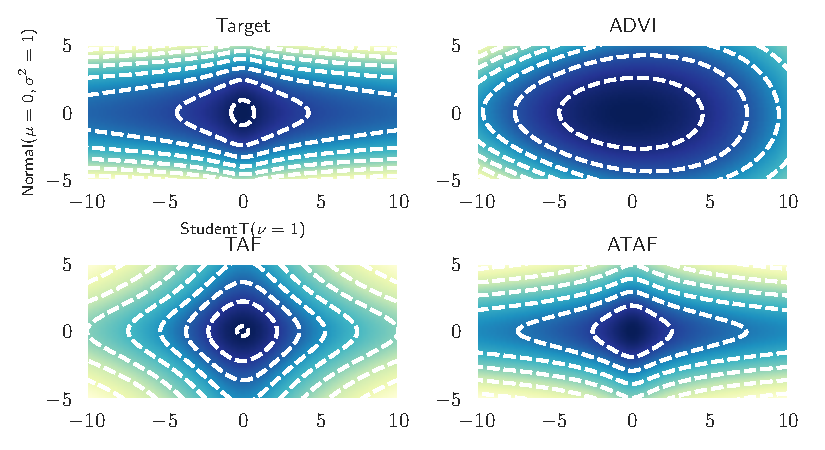
\includegraphics{../Figures/pancake.pdf}
    \vspace{-5mm}
  \caption{
    Variational inference against a tail-anisotropic target distribution $\cN(0,1) \otimes \text{StudentT}(\nu=1)$ (top left).
    Only ATAF (bottom right) is able to correctly reproduce the tail-anisotropy (fat-tailed along $x$-axis,
    Gaussian along $y$-axis).
    In contrast, ADVI's (top right) Gaussian base distribution and TAF's (bottom left) tail-isotropic $\prod_{i=1}^2 \text{StudentT}(\nu)$
    base distribution  can only model tail-isotropic distributions (\Cref{prop:isotropic-pushforward}),
    which erroneously imposes power-law tails with the same rate of decay along both the $x$ and $y$ axes.
    \vspace{-5mm}
  }
  \label{fig:pancake}
\end{figure*}

Our work here aims to identify and address these deficiencies.
To understand the impact of the base distribution $\mu$ in flow-based models,
we develop and apply theory for fat-tailed random variables and their transformations under Lipschitz-continuous functions.
Our approach leverages the theory of concentration functions \citep[Chapter 1.2]{ledoux2001concentration} to sharpen significantly and extend prior results
\citep[Theorem 4]{jaini2019sum} by describing precisely the tail parameters of the pushforward distribution $(f_\theta)_\ast \mu$ under both Lipschitz-continuous (\Cref{thm:distn_class_closed}) and polynomial (\Cref{corr:closure_polynomials}) transport maps.
% \michael{We say ``characterize'' but what do we mean.  Probably this is the place to say that it is particularly important to be flexible to have different tail indices in different directions.  Then some of the later sentences will make sense.}
%In the multivariate setting, we observe that it is important to be flexible and allow for a multivariate distribution
%to have different tail parameters in different directions. %Accordingly,
In the multivariate setting,
we develop a theory of direction-dependent tail parameters (\Cref{def:mv-tail-param}), and we show that tail-isotropic base distributions yield tail-isotropic pushforward measures (\Cref{prop:isotropic-pushforward}). 
As a consequence of \Cref{prop:isotropic-pushforward}, prior methods \citep{jaini2020tails} are limited in that
they are unable to capture \emph{tail-anisotropy}.
This motivates the construction of \emph{anisotropic tail adaptive flows} (ATAF, \Cref{def:ataf}) as a means to
alleviate this issue (\Cref{remark:anisotropic}) and to improve modeling of tail-anisotropic distributions.
% \michael{What limitation is precisely being referred to, since in the previous sentence we say that we get several results in this paper, and then we say how our results are a limitation.  Probably the best way to do this is to be more detailed, e.g., say that our \Cref{prop:isotropic-pushforward} means that the mapping can't introduce anisotropy.}
Our experiments show that ATAF exhibits correct tail behaviour in synthetic target distributions exhibiting fat-tails (\Cref{fig:cauchy_normal_student} of \Cref{sec:cauchy_normal_student}) and tail-anisotropy (\Cref{fig:pancake}).
On realistic targets,
% prior work \citep[Table 2]{jaini2020tails} showed tail-adaptive flows (TAF, a subset of ATAF)
% can improve density modeling and 
we find that ATAF can yield improvements in variational inference (VI) by capturing potential tail-anisotropy (\Cref{sec:experiments}).
% \michael{That sentence sounds like we are a footnote on them.  I would say that we get results for a ragne of cases, both for isotropic and anisotropic cases, thereby improving prior work that considered Gaussian things as well as prior work from \cite{jaini2020tails} that considered isotropic HT.}
\vspace{-3mm}
\subsection*{Related Work}
\vspace{-1mm}
\paragraph{Fat-Tails in Variational Inference.}

% The bulk of related work focuses on fat-tails arising from relaxing priors.
Recent work in variational autoencoders (VAEs) have considered relaxing Gaussian assumptions to heavier-tailed distributions \citep{mathieu2019disentangling,chen2019residual,boenninghoff2020variational,abiri2020variational}.
In \citet{mathieu2019disentangling}, a StudentT prior distribution $p(z)$ is considered over the latent code
$z$ in a VAE with Gaussian encoder $q(z \mid x)$. They argue
%\footnote{\url{https://github.com/iffsid/disentangling-disentanglement/blob/3396d40f46c34dd928a1241f567a86276b0ff41b/src/main.py\#L52}},
that the anisotropy of a StudentT product distribution leads to more disentangled representations, as compared to the standard choice of Normal distributions.
A similar modification is performed in \citet{chen2020use} for
a coupled VAE \citep{cao2019coupled}. 
This result showed improvements in the marginal
likelihoods of reconstructed images. In addition,
\citet{boenninghoff2020variational} consider a mixture of StudentTs for the
prior $p(z)$. To position
our work in context, note that the encoder $q(z \mid x)$ may be viewed
as a variational approximation to the posterior $p(z \mid x)$ defined by the
decoder model $p(x \mid z)$ and the prior $p(z)$. Our work differs from
\citet{mathieu2019disentangling,chen2020use,boenninghoff2020variational}, in
that we consider fat-tailed variational approximations $q(z \mid x)$ rather
than priors $p(z)$. Although \citet{abiri2020variational} also considers
a StudentT approximate posterior, our work involves a more general
variational family which uses normalizing flows.
% Relaxation of priors to heavy-tailed distributions has numerous
% applications beyond VAEs. In \cite{silnova2018fast}, the authors perform
% inference in heavy-tailed probabilistic linear discriminant analysis
% using Gaussian mean-field variational inference and show improved
% accuracy in speaker identification. Our work is complementary to these approaches;
% whereas they consider heavy-tailed priors $p(z)$ we consider heavy-tailed
% variational families $q(z \mid x)$.
Similarly, although \citet{wang2018variational} also deals with fat-tails in variational inference,
their goal is to improve $\alpha$-divergence VI by controlling the moments of importance
sampling ratios (which may be heavy-tailed). Our work here adopts
Kullback-Leibler divergence and is concerned with enriching the variational family
to include anisotropic fat-tailed distributions.
More directly comparable recent work \citep{ding2011t,futami2017expectation} studies the $t$-exponential family
variational approximation which includes StudentTs and other
heavier-tailed densities. Critically, the selection of their parameter $t$ (directly related to the
StudentT's degrees of freedom $\nu$), and the issue of tail anisotropy, are not discussed. %Other differences include their derivation of
%expectation-propagation update equations while 
% We directly backpropagate a noisy
% ELBO estimate, and introduce a richer variational family used by ATAF.

\vspace{-1mm}
\paragraph{Flow-Based Methods.}

Normalizing flows and other flow-based methods have a rich history within variational
inference \citep{kingma2016improved,rezende2015variational,agrawal2020advances,webb2019improving}.
Consistent with our experience (\Cref{fig:blr-anisotropic}), \citet{webb2019improving}
documents normalizing flows can offer improvements over ADVI and NUTS across thirteen different
Bayesian linear regression models from \citet{gelman2006data}.
\citet{agrawal2020advances} shows that normalizing flows compose nicely with other
advances in black-box VI (e.g., stick the landing, importance weighting).
However, none of these works treat the issue of fat-tailed targets and inappropriate tail
decay.
To our knowledge, only TAFs \citep{jaini2020tails} explicitly consider flows with tails
heavier than Gaussians. Our work here can be viewed as a direct improvement of \citet{jaini2020tails},
and we make extensive comparison to this work throughout the body of this paper. At
a high level, we provide a theory for fat-tails which is sensitive to the rate of
tail decay and develop a framework to characterize and address the tail-isotropic limitations plaguing
TAFs.

\vspace{-2mm}
\section{Flow-Based Methods for Fat-Tailed Variational Inference}

%Continuing from the notation introduced in \Cref{sec:intro}, in this section we
%finish establishing the VI setting and definitions/notation
%\michael{I'm not sure what ``Continuing ...'' means.  Can we say ``In this section we do such-and such ...".  Maybe something like:
%``In this section, we provide background on flow-vased methods for VI, and we describe some of the issues that arise when dealing with fat-tailed data and fat-tailed VI that will be important for understanding our main results. 
%}

\vspace{-2mm}
\subsection{Flow-Based VI Methods} 

The objective of VI is to approximate a target distribution $\pi(x)$ by searching over
a \emph{variational family} $\cQ = \{q_\phi : \phi \in \Phi\}$ of probability distributions $q_\phi$.
While alternatives exist \citep{li2016variational,wang2018variational}, VI typically
seeks to find $q_\phi$ ``close'' to $\pi$, as measured by Kullback-Leibler divergence $\infdiv{q_\phi}{\pi}$.
To ensure tractability without sacrificing generality, in practice \citep{wingate2013automated,ranganath2014black}
a Monte-Carlo approximation of the evidence lower bound (ELBO) is maximized:
\begin{align*}
  %-\infdiv{q_\phi}{\pi}
  %\propto 
  \text{ELBO}(\phi)
  &= \int q_\phi(x) \log \frac{\bar\pi(x)}{q_\phi(x)} dx\\
  & \approx \frac{1}{n} \sum_{i=1}^n \log \frac{\bar\pi(x_i)}{q_\phi(x_i)},\;
  x_i \simiid q_\phi,\;
  \bar{\pi} \propto \pi. 
\end{align*}
To summarize, this procedure enables tractable black-box VI
by replacing $\pi$ with $\bar\pi \propto \pi$ and approximating expectations with respect to $q_\phi$ (which are tractable only in simple variational families) through Monte-Carlo approximation. In Bayesian inference and probabilistic programming applications, the target posterior
$\pi(x) = p(x \mid y) = \frac{p(x, y)}{p(y)}$ is typically intractable but
$\bar\pi(x) = p(x,y)$ is computable (i.e., represented by the probabilistic program's
generative / forward execution).


\begin{table*}
  \centering
  \begin{tabular}{ccc}
    \toprule
    Model                                  & Autoregressive transform                                                                              & Suff. cond. for Lipschitz-continuity        \\
    \midrule
    NICE\citep{dinh2014nice}               & $z_j + \mu_j \cdot \mathds{1}_{k \not \in [j]}$                                                       & $\mu_j$ Lipschitz                      \\
    MAF\citep{papamakarios2017masked}      & $\sigma_j z_j + (1 - \sigma_j) \mu_j$                                                                 & $\sigma_j$ bounded                     \\
    IAF\citep{kingma2016improved}          & $z_j \cdot \exp(\lambda_j) + \mu_j$                                                                   & $\lambda_j$ bounded, $\mu_j$ Lipschitz \\
    Real-NVP\citep{dinh2016density}        & $\exp(\lambda_j \cdot \mathds{1}_{k \not\in[j]}) \cdot z_j + \mu_j \cdot \mathds{1}_{k \not \in [j]}$ & $\lambda_j$ bounded, $\mu_j$ Lipschitz \\
    Glow\citep{kingma2018glow}             & $\sigma_j \cdot z_j + \mu_j \cdot \mathds{1}_{k \not\in [j]}$                                         & $\sigma_j$ bounded, $\mu_j$ Lipschitz  \\
    NAF\citep{huang2018neural}             & $\sigma^{-1}(w^\top \cdot \sigma(\sigma_j z_j + \mu_j))$                                              & Always \par (logistic mixture CDF)          \\
    NSF\citep{durkan2019neural}            & $z_j \mathds{1}_{z_j \not\in [-B,B]} + M_j(z_j;z_{<j}) \mathds{1}_{x_j \in [-B,B]}$         & Always \par (linear outside $[-B,B]$)     \\
    FFJORD\citep{grathwohl2018ffjord} & n/a (not autoregressive)                                                                              & Always \par (required for invertibility)    \\
    ResFlow\citep{chen2019residual} & n/a (not autoregressive)                                                                              & Always \par (required for invertibility)    \\
    \bottomrule
  \end{tabular}
  \caption{Some popular / recently developed flows, the autoregressive transform used in the flow (if applicable),
  and sufficient conditions conditions for Lipschitz-continuity. A subset of this table was first presented
  in \citet{jaini2020tails}. $M(\cdot)$ denotes monotonic rational quadratic splines \citep{durkan2019neural}.
  \vspace{-5mm}
  }
  \label{tab:flows}
\end{table*}


While it is possible to construct a variational family $\cQ$ tailored to a specific task, we are interested in VI methods which are more broadly applicable and convenient to use: $\cQ$ should be automatically constructed from introspection of a given probabilistic model/program.
Automatic differentiation variational inference (ADVI, \citet{kucukelbir2017automatic}) is an early implementation of automatic VI and it is still the default in certain probabilistic programming languages \citep{carpenter2017stan}.
ADVI uses a Gaussian base distribution $\mu$ and a transport map $f_\theta = f \circ \Phi_\text{Affine}$ comprised of an invertible affine transform composed with a deterministic transformation $f$ from $\RR$ to the target distribution's support (e.g., $\exp : \RR \to \RR_{\geq 0}$, $\text{sigmoid} : \RR \to [0,1]$).
As Gaussians are closed under affine transformations, ADVI's representational capacity is limited to deterministic transformations of Gaussians. Hence it cannot represent complex multi-modal distributions.
To address this, more recent work \citep{kingma2016improved,webb2019improving} replaces the affine map $\Phi_\text{Affine}$ with a flow $\Phi_{\text{Flow}}$ typically parameterized by an invertible neural network:
\begin{definition}
    \label[definition]{def:advi}
  ADVI (with normalizing flows) comprise the variational family
  $\cQ_\text{ADVI}~\coloneqq~\{
    (f~\circ~\Phi_\text{Flow})_\ast \mu
    \}$, 
  where $\mu = \text{Normal}(0_d, I_d)$,
  $\Phi_\text{Flow}$ is an invertible flow transform (e.g., \Cref{tab:flows})
  and $f$ is a deterministic bijection between constrained supports \citep{kucukelbir2017automatic}.
\end{definition}


As first noted in \citet{jaini2020tails}, the pushforward of a light-tailed Gaussian base distribution under a Lipschitz-continuous flow will remain light-tailed and provide poor approximation to fat-tailed targets. 
Despite this, 
%at the time of writing this paper 
many major probabilistic programming packages still make a default choice of Gaussian base distribution (\texttt{AutoNormalizingFlow}/\texttt{AutoIAFNormal} in Pyro \citep{bingham2019pyro}, \texttt{method=variational} in Stan \citep{carpenter2017stan}, \texttt{NormalizingFlowGroup} in PyMC \citep{patil2010pymc}).
%\michael{What is the verb in the following sentence}
To address this issue, tail-adaptive flows \citep{jaini2020tails} use a
base distribution $\mu_\nu = \prod_{i=1}^d \text{StudentT}(\nu)$,
where a single degrees-of-freedom $\nu \in \RR$ is used across all $d$ dimensions. Here is a more precise definition.
\begin{definition}
  \label[definition]{def:taf}
  Tail adaptive flows (TAF) comprise the variational family
  $\cQ_\text{TAF}
    \coloneqq \{
    (f \circ \Phi_\text{Flow})_\ast \mu_\nu
    \}$,
  where $\mu_\nu = \prod_{i=1}^d \text{StudentT}(\nu)$ with $\nu$ shared across all $d$ dimensions,
  $\Phi_{\text{Flow}}$ is an invertible flow,
  and $f$ is a bijection between constrained supports \citep{kucukelbir2017automatic}.
  During training, the shared degrees of freedom $\nu$ is treated as an additional variational parameter.
\end{definition}


\vspace{-2mm}
\subsection{Fat-Tailed Variational Inference}

\vspace{-1mm}
Fat-tailed variational inference (FTVI)
% \michael{I'm inclined to say that we should have ``(FTVI)'' and then refer to that acronym everywhere; then we can say: VI is important, FTVI is very important, ADVI did a good job with FTVI, we do a great job with FTVI, and you the reader should follow up on us and do FTVI.  It's the sort of acronym that is nice to remember.}
% will do, and add this discussion to future directions in conclusion
considers the setting where the target $\pi(x)$ is fat-tailed. 
Such distributions commonly arise during a standard
``robustification'' approach where light-tailed noise distributions are
replaced with fat-tailed ones \citep{tipping2005variational}. They also
appear when weakly informative prior distributions are used in Bayesian
hierarchical models \citep{gelman2006prior}.




To formalize these notions of fat-tailed versus light-tailed distributions, a quantitative classification for tails is required.
While prior work classified distribution tails according to quantiles and the existence of moment generating functions
\citep[Section 3]{jaini2020tails}, here we propose a more natural and finer-grained classification based upon
the theory of concentration functions \citep[Chapter 1.2]{ledoux2001concentration}, which is sensitive to
the rate of tail decay.

\begin{definition}[Classification of tails]
    \label[definition]{def:tail-classification}
    For each $\alpha,p > 0$, we let 
    \vspace{-1mm}
    \begin{itemize}[leftmargin=*]
        \item $\mathcal{E}_\alpha^p$ denote the set of \emph{exponential-type} random variables $X$ with $\mathbb{P}(|X| \geq x) = \Theta(e^{-\alpha x^p})$;
    \vspace{-1mm}
        \item $\mathcal{L}_\alpha^p$ denote the set of \emph{logarithmic-type} random variables $X$ with $\mathbb{P}(|X| \geq x) = \Theta(e^{-\alpha(\log x)^p})$.
    \end{itemize}
    \vspace{-1mm}
    % A random variable $X$ is of %\textbf{exponential-type}, denoted $X \in \cE_\alpha^p$, w
    % \begin{description}
    %     \item[exponential-type], denoted $X \in \cE_\alpha^p$,
    %   whenever $\PP(\lvert X \rvert \geq x) = \Theta(e^{-\alpha x^p})$, and
    %     \item[logarithmic-type], denoted $X \in \cL^p_\alpha$, whenever $\PP(\lvert X \rvert \geq x) = \Theta(e^{-\alpha (\log x)^p})$.
    % \end{description}
    In both cases, we call $p$ the \emph{class index} and $\alpha$ the \emph{tail parameter} for $X$.
    Note that every $\cE_\alpha^p$ and $\cL_\beta^q$ are disjoint, that is,
    $\cE_\alpha^p \cap \cL_\beta^q = \emptyset$ for all $\alpha,\beta,p,q > 0$.
    For brevity, we define the ascending families
    $\overline{\cE_\alpha^p}$ and $\overline{\cL_\alpha^p}$
    analogously as before except with $\Theta(\cdot)$ replaced
    by $\cO(\cdot)$. Similarly, we denote the class of distributions with exponential-type
    tails with class index at least $p$
    by $\overline{\cE^p} = \cup_{\alpha \in \RR_+} \overline{\cE_\alpha^p}$, and similarly for $\overline{\cL^p}$.
\end{definition}

For example, $\overline{\cE_\alpha^2}$ corresponds to $\alpha^{-1/2}$-sub-Gaussian random variables,
    $\overline{\cE_\alpha^1}$ corresponds to sub-exponentials, and (of particular relevance to this paper) $\cL^1_\alpha$ corresponds to the class of power-law distributions.

\vspace{-2mm}
\section{Tail Behavior of Lipschitz Flows}

\vspace{-1mm}
This section states our main theoretical contributions; proofs are deferred to \Cref{sec:proofs}.
We sharpen previous impossibility results approximating fat-tailed targets
using light-tailed base distributions \citep[Theorem 4]{jaini2020tails}
by characterizing the effects of Lipschitz-continuous transport maps on not only the tail class
but also the class index and tail parameter (\Cref{def:tail-classification}). Furthermore, we extend the theory
to include polynomial flows \citep{jaini2019sum}. For the multivariate setting,
we define the tail-parameter function (\Cref{def:mv-tail-param}) to help formalize the notion
of tail-isotropic distributions and prove a fundamental limitation that tail-isotropic
pushforwards remain tail-isotropic (\Cref{prop:isotropic-pushforward}).

Most of our results are developed within the context of Lipschitz-continuous transport maps $f_\theta$.
In practice, many flow-based methods exhibit Lipschitz-continuity in their transport map, either by design \citep{grathwohl2018ffjord,chen2019residual}, or as a consequence of choice of architecture and activation function (\Cref{tab:flows}). % or by being enforced stemming from the Banach fixed point theorem 
%
%or .
The following assumption encapsulates this premise.
\begin{assumption}\label[assumption]{assump:lipschitz}
    $f_\theta$ is invertible, and both $f_\theta$ and $f^{-1}_\theta$
    are $L$-Lipschitz continuous (e.g., sufficient conditions in \Cref{tab:flows} are satisfied).
\end{assumption}
It is worth noting that domains other than $\mathbb{R}^d$ may require an additional bijection between supports (e.g. $\exp : \mathbb{R} \to \mathbb{R}_+$) which
could violate \cref{assump:lipschitz}.

\vspace{-2mm}
\subsection{Closure of Tail Classes}
\label{ssec:failure}

\vspace{-1mm}
Our first set of results pertains to the closure of the tail classes in \Cref{def:tail-classification}
under Lipschitz-continuous transport maps. While earlier work \citep{jaini2020tails} demonstrated
closure of exponential-type distributions $\cup_{p > 0} \overline{\cE^p}$ under flows satisfying \Cref{assump:lipschitz}, our results in Theorem \ref{thm:distn_class_closed} and Corollaries \ref{corr:heavy_to_light} and \ref{corr:closure_polynomials} sharpen these observations, showing that: (1) Lipschitz transport maps cannot decrease the class index $p$ for exponential-type random variables, but they can alter the tail parameter $\alpha$; and
(2) under additional assumptions, they cannot change either class index $p$ or the tail parameter $\alpha$ for logarithmic-type random variables.
%         tail parameter $\alpha$; 
% \begin{itemize}[leftmargin=*]
%     \item cannot decrease the class index $p$ for exponential-type random variables, but can alter the
%         tail parameter $\alpha$; and
%     \item under additional assumptions, cannot change either class index $p$ or the tail
%         parameter $\alpha$ for logarithmic-type random variables.
% \end{itemize}

\begin{theorem}[Lipschitz maps of tail classes]
  \label{thm:distn_class_closed}
  Under \Cref{assump:lipschitz},
  the distribution classes $\overline{\cE^p}$
  and $\overline{\cL^p_\alpha}$ (with $p,\alpha > 0$) are closed
  under every flow transformation in \Cref{tab:flows}.
\end{theorem}

Informally, \Cref{thm:distn_class_closed} asserts that light-tailed base distributions cannot be transformed
via Lipschitz transport maps into fat-tailed target distributions.
Note this does not violate universality theorems for certain flows \citep{huang2018neural}
as these results only apply in the infinite-dimensional limit. Indeed, certain exponential-type families (such as Gaussian mixtures) are dense in the class of \emph{all} distributions, including those that are fat-tailed.

Note that $\overline{\cL^p_\alpha} \supset \cE^q_\beta$ for all $p,q,\alpha,\beta$, so \Cref{thm:distn_class_closed}
by itself does not preclude transformations of fat-tailed base distributions to light-tailed targets.
Under additional assumptions on $f_\theta$, we further establish a partial converse that a fat-tailed base distribution's tail parameter is unaffected after pushfoward,
hence heavy-to-light transformations are impossible. Note here there is no ascending union over
tail parameters (i.e., $\cL^p_\alpha$ instead of $\overline{\cL^p_\alpha}$).

\begin{corollary}[Closure of $\cL^p_\alpha$]
  \label[corollary]{corr:heavy_to_light}
  If in addition $f_\theta$ is smooth
  with no critical points on the interior or boundary of
  its domain, then $\cL_\alpha^p$ is closed.
\end{corollary}

This implies that simply fixing a fat-tailed base
distribution \emph{a priori} is insufficient; the tail-parameter(s) of the base distribution must be explicitly optimized alongside
the other variational parameters during training.
While these additional assumptions may seem restrictive, note that many flow transforms
explicitly enforce smoothness and monotonicity \citep{wehenkel2019unconstrained,huang2018neural,durkan2019neural}
and hence satisfy the premises. In fact, we can show a version of \Cref{thm:distn_class_closed} ensuring closure of exponential-type
distributions under polynomial transport maps which do not satisfy \Cref{assump:lipschitz}.
This is significant because it extends the closure results to
include polynomial flows such as sum-of-squares flows \citep{jaini2019sum}.

\begin{corollary}[Closure under polynomial maps]
    \label[corollary]{corr:closure_polynomials}
  For any $\alpha, \beta, p, q \in \RR_+$, there does not exist a
  finite-degree polynomial map from $\cE_\alpha^p$ into $\cL_\beta^q$.
\end{corollary}

% Suffices to show for k \in \RR_{> 0}, this covers inverse powers

% \begin{remark}
%   There does not exist a inverse polynomial map (e.g., sqrt) from $\cL_\alpha$ to $\cE$.
% \end{remark}

\vspace{-2mm}
\subsection{Multivariate Fat-Tails and Anisotropic Tail Adaptive Flows}

\vspace{-1mm}
Next, we restrict attention to power-law tails $\cL^1_\alpha$, and we develop a multivariate fat-tailed theory and notions of isotropic/anisotropic tail indices. Using our theory, we prove that both ADVI and TAF are fundamentally limited because they
are only capable of fitting tail-isotropic target measures (\Cref{prop:isotropic-pushforward}).
We consider anisotropic tail adaptive flows (ATAF): a density
modeling method which can represent tail-anisotropic distributions (\Cref{remark:anisotropic}).

% Karamata's theorem enables recovery of a regularly varying random variable's
% index: $X \in \cL^1_\alpha$ means that $\lim_{x \to \infty} \frac{x \PP(X \geq
%     x)}{\int_x^\infty \PP(X \geq t) dt} = \alpha$ for $\alpha < -1$.
% Motivated by Karamata's theorem, we introduce
% the following definition to aid in describing multivariate fat-tailed random variables:

For example, consider the target distribution shown earlier in \Cref{fig:pancake} formed as the product of $\mathcal{N}(0,1)$ and $\text{StudentT}(\nu=1)$ distributions.
The marginal/conditional distribution along a horizontal slice (e.g., the distribution of $\braket{X,e_0}$)
is fat-tailed, while along a vertical slice (e.g., $\braket{X,e_1}$) it is Gaussian.
Another extreme example of tail-anisotropy where the tail parameter for
$\braket{X,v}$ is different in every direction $v \in \cS^{1}$
is given in \Cref{fig:radial-fat-tail}. Here $\mathcal{S}^{d-1}$ denotes the $(d-1)$-sphere in $d$ dimensions. 
Noting that the tail parameter depends on the choice of direction, we are motivated to consider
the following direction-dependent definition of multivariate tail parameters. 

\begin{definition}
  \label[definition]{def:mv-tail-param}
  For a $d$-dimensional random vector $X$,
  its \emph{tail parameter function} $\alpha_X : \cS^{d-1} \to \bar{\RR}_+$
  is defined as
  % $\alpha_X(v) = \lim_{x \to \infty} \frac{x \PP(\braket{v,X} \geq x)}{\int_x^\infty \PP(\braket{v,X} \geq t) dt}$.
  $\alpha_X(v) = -\lim_{x \to \infty} \log \PP(\braket{v,X} \geq x) / \log x$ when the limit exists, and $\alpha_X(v) = +\infty$ otherwise.
  In other words, $\alpha_X(v)$ maps directions $v$ into the tail parameter of the corresponding one-dimensional projection $\braket{v,X}$. The random vector $X$ is \emph{tail-isotropic} if $\alpha_X(v) \equiv c$ is constant and
  \emph{tail-anisotropic} if $\alpha_X(v)$ is not constant but bounded.
\end{definition}


\begin{figure*}[htbp]
  \centering
  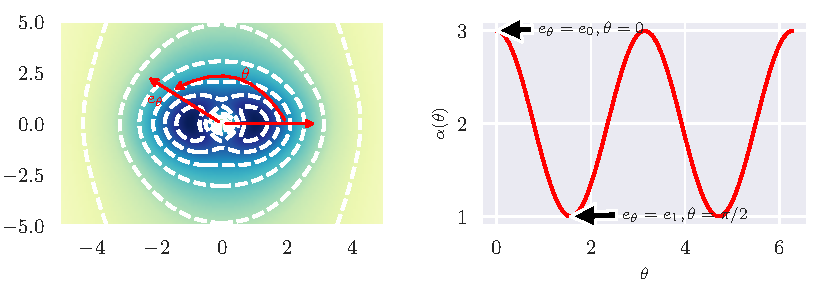
\includegraphics{../Figures/radial-fat-tail.pdf}%
%   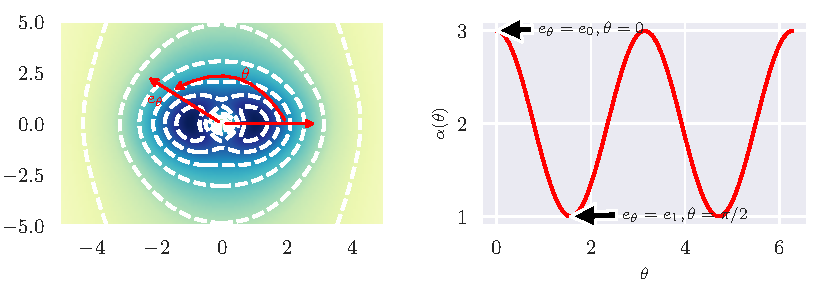
\includegraphics[trim={0 0 7cm 0},clip]{../Figures/radial-fat-tail.pdf}\\%
%   \vspace{-8mm}
%   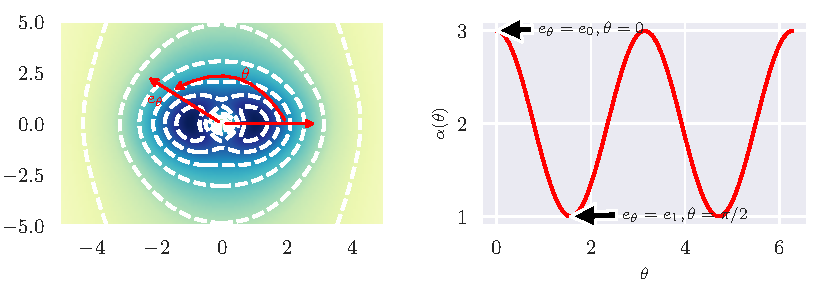
\includegraphics[trim={7.2cm 0 0 0},clip]{../Figures/radial-fat-tail.pdf}%
  %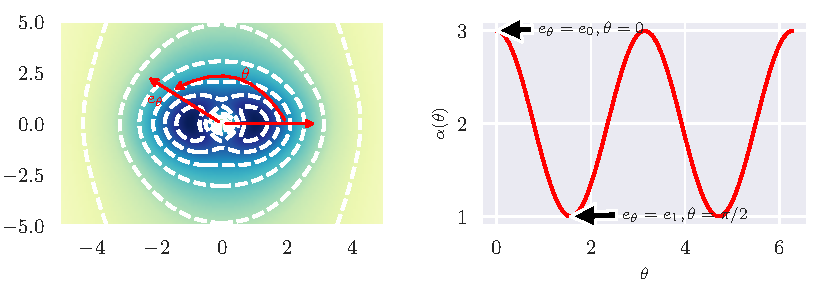
\includegraphics[width=\textwidth]{../Figures/radial-fat-tail.png}%
  %\input{../Figures/radial-fat-tail.pgf}
  \vspace{-7mm}
  \caption{
    Illustration of the direction-dependent tail-parameter function (right) on a tail-anisotropic distribution (left)
    with PDF $\dd P(r,\theta) = r^{-\alpha(\theta)} r \dd r \dd\theta$ and tail parameter $\alpha(\theta) = 2 + \cos(2\theta)$.
    While prior fat-tailed theory based on $\|X\|_2 = \sup_{\|v\|_2 = 1} \braket{X,v}$
    is only sensitive to the largest tail parameter $\max_{\theta \in [0, 2\pi]} \alpha(\theta) = 3.0$,
    our direction-dependent tail parameter function (bottom, red line)
    and its values along the standard basis axes ($\alpha(0)$ and $\alpha(\pi/2)$)
    capture \emph{tail-anisotropy}.
    \vspace{-5mm}
  }
  \label{fig:radial-fat-tail}
\end{figure*}
% \begin{definition}
%   \label[definition]{def:isotropic}
%   Multivarate random variable $X$ is tail-isotropic if $\alpha_X(v) \equiv c$ is constant.
%   Otherwise, it is tail-anisotropic.
% \end{definition}


% \begin{align*}
%   \PP[\braket{X,u} \geq x]
%   = \PP[\braket{\mu,u} + R \braket{AU,u} \geq x]
%   = \PP[R \geq \frac{x - \braket{\mu,u}}{\braket{u,AU}}]
%   \sim C_1 \left(\frac{x - \braket{\mu,u}}{\braket{u,AU}}\right)^{-\alpha}
%   \sim C_2 x^{-\alpha}
% \end{align*}
% and
% theory around tail parameters is developed for elliptically
% contoured multivariate distributions $X = \mu + R A U$
% for some heavy-tailed random variable $R$, fixed vectors $\mu \in \RR^d$
% and $U \in S^{d-1}$, and $A$ a (Cholesky factor)
% defining the ellipsoid axes.

% While elliptically contoured multivariate distributions admit a
% straightforward generalization from the scalar case, they are severely
% limited in practical applications.  One fundamental limitation of
% elliptically contoured $X$ is that the tail parameter is the same for every
% 1-dimension projection.  If $R$ has tail index $\alpha$ then for all for $u
%   \in S^{d-1}$
% \begin{align*}
%   \PP[\braket{X,u} \geq x]
%   = \PP[\braket{\mu,u} + R \braket{AU,u} \geq x]
%   = \PP[R \geq \frac{x - \braket{\mu,u}}{\braket{u,AU}}]
%   \sim C_1 \left(\frac{x - \braket{\mu,u}}{\braket{u,AU}}\right)^{-\alpha}
%   \sim C_2 x^{-\alpha}
% \end{align*}

% Furthermore, the assumption of elliptical distributions are
% easily violated in many common and useful applications.  For example, in
% probabilistic programming collections of random variables are oftentimes
% grouped together into a single multivariate random variable (e.g.,  blocked
% Gibbs, Hamiltonian Monte Carlo).  In fact, $Q_{TAF}$ (used in the experiments
% in \citep{jaini2020tails}) uses a StudentT product base distribution which
% is not elliptically symmetric.

% \begin{figure}[htbp]
%   \centering
%   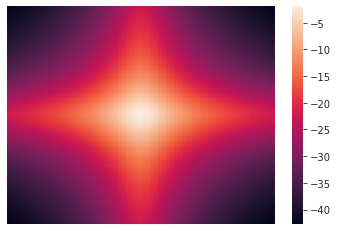
\includegraphics[width=0.4\textwidth]{../Figures/studentt-product.png}
%   \caption{
%     Illustrating multivariate fat-tails using a 2-dimensional StudentT.
%     The multivariate theory from \citep{jaini2020tails} is for elliptically
%     contoured distributions and not applicable to the StudentT product base distributions
%     used in their experiments.
%   }
%   \feynman{Consider just using words here to delineate from our contributions, this is not a super important fact}
%   \label{fig:studentt-product}
% \end{figure}




% Elliptical distributions are \emph{tail isotropic} i.e., $\alpha(v) \equiv c$ is constant.
% The base distribution for \citep{jaini2020tails}, $\prod_1^d \text{StudentT}(\nu_i)$ with $\nu_i \equiv \nu$,
% is also tail isotropic because
% $\braket{v,X}$ is a sum of StudentT and by tail index algebra
% has index $\max_i \nu_i = \nu$.
Of course, one can construct pathological densities where this definition is not effective
(see \Cref{eg:spiral}), but it will suffice for our purposes. 
It is illustrative to contrast with the theory presented for TAF \citep{jaini2020tails},
where only the tail exponent of $\|X\|_2$ is considered.
For $X = (X_1, \ldots, X_d)$ with $X_i \in \cL^1_{\alpha_i}$, 
by Fatou-Lebesgue and \Cref{lem:sum-rule}
\begin{align*}
  &\PP[\|X\|_2 \geq t]
  = \PP\left[\sup_{z \in \cS^{d-1}} \braket{X,z} \geq t\right]\\
  &\quad \geq \sup_{z \in \cS^{d-1}} \PP[\braket{X,z} \geq t]
  = \max_{1 \leq i \leq d} \nu_i
  = \max_{0 \leq i \leq d-1} \alpha_X(e_i) .
\end{align*}
Therefore, considering only the tail exponent of $\|X\|_2$ is equivalent to summarizing $\alpha_X(\cdot)$ by an upper bound.
Given the absence of the tail parameters for other directions (i.e., $\alpha_X(v) \neq \sup_{\|v\|=1} \alpha_X(v)$)
in the theory for TAF \citep{jaini2020tails}, it should be unsurprising that both their multivariate 
theory as well as their experiments only consider tail-isotropic distributions obtained either
as an elliptically-contoured distribution with fat-tailed radial distribution or 
$\prod_{i=1}^d \text{StudentT}(\nu)$ (tail-isotropic by \Cref{lem:sum-rule}). 
Our next proposition shows that this presents a significant limitation when the target distribution is
tail-anisotropic.


\begin{proposition}[Pushforwards of tail-isotropic distributions]
  \label[proposition]{prop:isotropic-pushforward}
  Let $\mu$ be tail isotropic with non-integer parameter $\nu$
  and suppose $f_\theta$ satisfies \Cref{assump:lipschitz}.
  Then $(f_\theta)_\ast \mu$ is tail isotropic with parameter $\nu$.
\end{proposition}

% However, $\alpha(v)$ is non-trivial to work with; it is an asymptotic quantity and is defined
% for uncountably many $v \in S^{d-1}$. In this work, we propose approximating
% $\alpha(v)$ using the standard basis vectors:

% \begin{definition}
%   The \emph{standard basis tail parameters} of a fat-tailed $X \in \RR^d$
%   is $\{\alpha(e_i) : i \in [d]\}$ where $\alpha$ is defined in
%   \Cref{def:mv-tail-param} and $e_i$ is the $i$th standard basis vector.
% \end{definition}

% The standard basis vectors provide a natural choice of projections for
% multivariate product distributions (as commonly encountered during blocking /
% grouping of random variables). Going back to our previous example,
% we still have that $\alpha_{\|X\|} = \max_i \alpha(e_i)$ but now the tail
% indices of the remaining $e_j$ need not be equal. Admittedly, the standard basis
% is less suitable for correlated multivariate distributions. For example,
% let $t_i \sim \text{StudentT}(\nu_i)$ and consider the rotated random variable
% $X = R_{\pi/4} [t_1; t_2]$. Its standard basis tail parameters are
% \begin{align*}
%   \Pr[\braket{X,e_1} > x]
%   = \Pr[\braket{X,e_2} > x]
%   = \Pr[0.5 t_1 + 0.5 t_2 > x]
%   \leq \max_i \nu_i
% \end{align*}
% This example illustrates that the standard basis tail parameters
% provide multivariate tail parameters which are no worse than
% previous work.

% \subsection{Limitations of our theory}

% \begin{itemize}
%   \item Standard basis parameters not general, only works for axis-aligned tails
%   i.e., independent product distributions
%   \item Still fails on the spiral, but it should do better than TAF
%   \item Theory not fully general, only considers rays from origin rather than
%   path integrals
% \end{itemize}

To work around this limitation without relaxing \Cref{assump:lipschitz}, it is evident
that tail-anisotropic base distributions $\mu$ must be considered. Perhaps the most straightforward modification to incorporate a tail-anisotropic base distribution replaces TAF's isotropic base distribution $\prod_{i=1}^d \text{StudentT}(\nu)$
with $\prod_{i=1}^d \text{StudentT}(\nu_i)$. Note that $\nu$ is no longer shared across dimensions,
enabling $d$ different tail parameters to be represented:

\begin{definition}\label[definition]{def:ataf}
  Anisotropic Tail-Adaptive Flows (ATAF) comprise the variational family
  $\cQ_\text{ATAF}~\coloneqq~\{
    (f \circ \Phi_\text{Flow})_\ast \mu_\nu
    \},$
  where $\mu_\nu = \prod_{i=1}^d \text{StudentT}(\nu_i)$, each $\nu_i$ is \emph{distinct}, and $f$ is a bijection between constrained supports \citep{kucukelbir2017automatic}.
  Analogous to \citet{jaini2020tails}, ATAF's implementation
  treats $\nu_i$ identically to the other parameters in the flow and jointly optimizes over them.
\end{definition}


\begin{remark}\label[remark]{remark:anisotropic}
  Anisotropic tail-adaptive flows can represent tail-anisotropic distributions with up to $d$ different
  tail parameters while simultaneously satisfying \Cref{assump:lipschitz}.
  For example, if $\Phi_\text{Flow} = \text{Identity}$ and $\mu_\nu = \prod_{i=1}^d \text{StudentT}(i)$
  then the pushforward $(\Phi_\text{Flow})_\ast \mu_\nu = \mu_\nu$ is tail-anisotropic.
  % Moreover, its standard basis tail parameters are equal
  % (up to permutation) to those for $\mu$.
\end{remark}

Naturally, there are other parameterizations of the tail parameters $\nu_i$ that may be more effective depending on the application. For example, in high dimensions, one might prefer not to allow for $d$ unique indices, but perhaps only fewer. On the other hand, by using only $d$ tail parameters, an approximation error will necessarily be incurred when more than $d$ different tail parameters are present. \Cref{fig:radial-fat-tail} presents a worst-case scenario where the target distribution has a continuum of tail parameters. In theory, this density could itself be used as an underlying base distribution, although we have not found this to be a good option in practice. The key takeaway is that to capture several different tails in the target density, one must consider a base distribution that incorporates sufficiently many \emph{distinct} tail parameters. 

Concerning the choice of StudentT families, we remark that since $\text{StudentT}(\nu) \Rightarrow \cN(0,1)$ 
as $\nu \to \infty$, ATAF should still provide reasonably good approximations to target 
distributions in $\overline{\cE^2}$ by taking $\nu$ sufficiently large. This can be seen in practice in \Cref{sec:normal-normal-location-mixture}.
%whereas the tail-parameter function may take on more than $d$ values. \Cref{fig:radial-fat-tail}
%presents a worst-case scenario.
%As ATAF is only capable of representing $d$ different tail parameters in its pushforward
%(\Cref{remark:anisotropic}), it will necessarily incur an approximation error when $> d$ different
%tail parameters are present.

% Compared to \citep{jaini2020tails}, the degrees of freedom $\nu$ is no longer
% shared across all $d$ dimensions so the variational approximations may exhibit
% varying degrees of fat-tailedness across different dimensions. As seen in
% \Cref{fig:pancake}, such anisotropy is particularly important in situations
% such as the ``heavy-tailed pancake.'' This situation is particularly relevant in
% probabilistic programming, where multiple latent variariables (potentially of different
% tail index) are blocked together for joint sampling / approximation.

%\vspace{-2mm}
%\subsection{Discussion of limitations}
%\label{ssec:limitations}

%\vspace{-1mm}
%By only considering projections $\braket{X,v}$ along rays through the origin
%$v \in \cS^{d-1}$, the limit in $\alpha_X(\cdot)$ may not be defined
%(see \cref{eg:spiral}).

%Furthermore, 
% We found that applying ATAF when the target is light tailed results in minimal
% error (\Cref{sec:normal-normal-location-mixture}); the result agrees with
% intuition because $\text{StudentT}(\nu) \to N(0,1)$ as $\nu \to \infty$ so
% it is reasonable to expect ATAF to learn reasonable approximations.

% \subsection{Non-parametric tail index estimation}
% \label{ssec:non-param-index}

% To perform variational inference with $\cQ_{ATAF}(\nu,\Phi)$, note that if
% $\Phi$ is Lipschitz then the tail index of any element of
% $\cQ_{ATAF}(\nu,\Phi)$ depends only on $\nu$. This motivates a two step
% procedure where (1) $\hat\nu$ estimates the degrees of freedom and
% (2) standard normalizing-flow variational inference $\max_\Phi \cQ_{ATAF}(\hat\nu,\Phi)$ is performed. The key advantage here is that both steps are standard,
% so existing techniques for tail index estimation may be applied.

% Let $X$ be a random variable with fat-tailed density $\pi(x)$
% with tail index $\alpha$ which we wish to estimate.
% When samples $X_i \simiid \pi$ are tractable
% (e.g., no \texttt{observe} or \texttt{condition} statements), traditional
% tail-index estimation techniques may be applied:

% \begin{figure}[H]
%   \centering
%   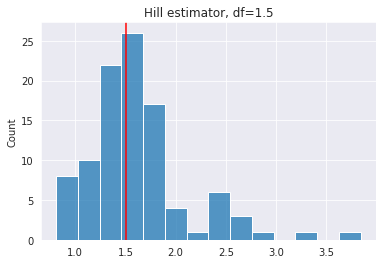
\includegraphics[width=0.6\textwidth]{../Figures/hill.png}
%   \caption{Hill estimator against $\nu=1.5$ StudentT}
%   \label{fig:hill}
% \end{figure}

% Oftentimes $\pi$ is the posterior distribution of latent variable $X$
% after conditioning on observations $Y=y$, in which case
% $\pi(x) = p(X=x \mid Y=y) = \frac{p(x,y)}{p(y)}$
% and sampling from $\pi$ is non-trivial.
% To circumvent this, we propose the following asymptotically correct
% estimator. Note for $a, b$ large:
% \begin{align*}
%   \Pr[X > a]                 & \sim b^{-\alpha}                                           \\
%   \pi(a)                     & \sim \alpha a^{-\alpha - 1}                                \\
%   \log \pi(a)                & \sim \log \alpha - (\alpha + 1) \log a                     \\
%   \log \frac{p(a,y)}{p(b,y)} & = \log \frac{\pi(a)}{\pi(b)}
%   \sim (\alpha + 1) \log \frac{b}{a}                                                      \\
%   \alpha                     & \sim \frac{\log p(a,y) - \log p(b,y)}{\log b - \log a} - 1
% \end{align*}
% The joint density $p(x,y)$ is tractably computed by running the
% probabilistic program forwards.
% For example. setting $a=10$ and $b=20$ yields an estimate of $1.4799$ for a
% $\nu=1.5$ StudentT.

% \subsubsection{Approximating 1D-marginals}

% This is an example of a two-point log-linear extrapolation at points $a$ and $b$.
% \feynman{Consider Richardson extrapolation to accelerate this limit. Rate of convergece in limit must be a power}

% In general, PPs may include several latent variables.
% The 1-dimensional marginal $p(x, y) = \int_{\setminus x} p(x,z,y) dz$
% is required to apply the above interpolation method.
% We propose approximating this integral using discrete samples.
% If $z$ is a descendent of $y$, then
% we can compute $p(x,y)$ by executing the probabilistic program
% (possibly terminating early).
% If $z$ is an ancestor of $x$ (hence also an ancestor of $y$), then
% \begin{align*}
%   p(x,y) \approx \frac{1}{N} \sum_{i=1}^N p(y, x \mid z_i)
%   \qquad z_i \simiid p(z)
% \end{align*}
% In the last case where $x \rightarrow z \rightarrow y$,
% we have
% \begin{align*}
%   p(x,y) \approx p(x) \frac{1}{N} \sum_{i=1}^n p(y \mid x, z_i)
%   \qquad z_i \simiid p(z_i \mid x)
% \end{align*}

% \begin{figure}[H]
%   \centering
%   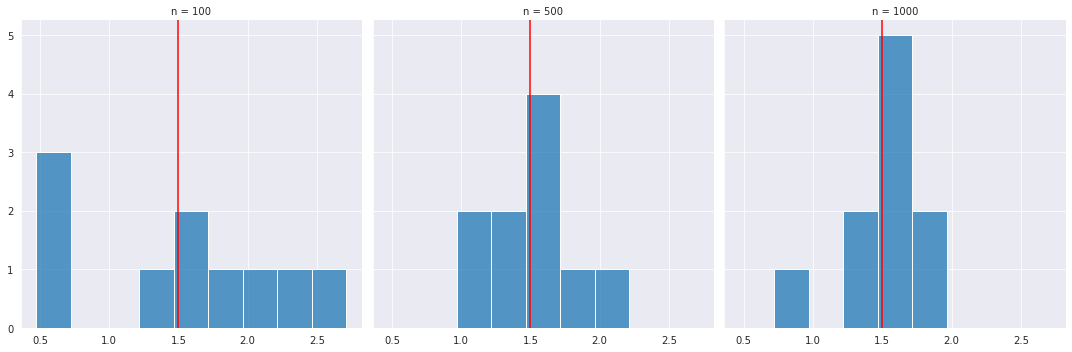
\includegraphics[width=0.9\textwidth]{../Figures/our-estimator.png}
%   \caption{Tail index estimation on location-scale mixture representation
%     for StudentT, where the mixture is discretized to $n$ components.}
%   \label{fig:approx_marg}
% \end{figure}

\vspace{-2mm}
\section{Experiments}
\label{sec:experiments}

\vspace{-1mm}
Here we validate ATAF's ability to improve
a range of probabilistic modeling tasks.
Prior work \citep{jaini2020tails} demonstrated improved
density modelling when fat tails are considered, and
our experiments are complementary by evaluating TAFs and ATAFs for variational inference tasks as well as by demonstrating the effect of tail-anisotropy for modelling real-world financial returns and insurance claims datasets.
We implement using the 
\texttt{beanmachine} probabilistic programming language \citep{tehrani2020bean}
%\texttt{REDACTED FOR REVIEW} probabilistic programming language[REDACTED]
and the
\texttt{flowtorch} library for normalizing flows \citep{flowtorchai},
%\texttt{REDACTED FOR REVIEW} library for normalizing flows[REDACTED],
%and we have open-sourced the code\citep{ghlic}
and we have open-sourced code for reproducing experiments in Supplementary Materials. 
% TODO: add facebookresearch reference 
Additional details for the experiments are detailed in \Cref{sec:additional-exp-details}.

% These experiments investigate the behavior of neural density estimators with
% \emph{heavy-tailed base distribution}.
% Specifically, we consider a masked autoregressive flow \cite{papamakarios2017masked}
% transform of a generalized Student's t distribution as a density estimator $q_\theta(X)$
% in a variational inference framework. To fit $q_\theta$ to a target distribution
% $\pi$, the ELBO gradient is reparameterized and Monte-Carlo approximated
% \begin{align*}
%   \nabla_\theta \EE_{q_\theta} \log \frac{\pi(X)}{q_\theta(X)}
%   & = \nabla_\theta \EE_p \log \frac{
%     \pi(X)
%   }{p_\theta(f_\theta^{-1}(X))
%   \left\lvert \det \nabla f_\theta^{-1}(X) \right\rvert}    \\
%   & = \EE_p \nabla_\theta \log \frac{
%     \pi(X)
%   }{p_\theta(f_\theta^{-1}(X))
%   \left\lvert \det \nabla f_\theta^{-1}(X) \right\rvert}    \\
%   & \approx \frac{1}{n} \sum_i^n \nabla_\theta \log \frac{
%     \pi(x_i)
%   }{p_\theta(f_\theta^{-1}(x_i))
%     \left\lvert \det \nabla f_\theta^{-1}(x_i) \right\rvert}
% \end{align*}

\begin{figure*}[htbp]
  \centering
  \vspace{-0.2cm}
  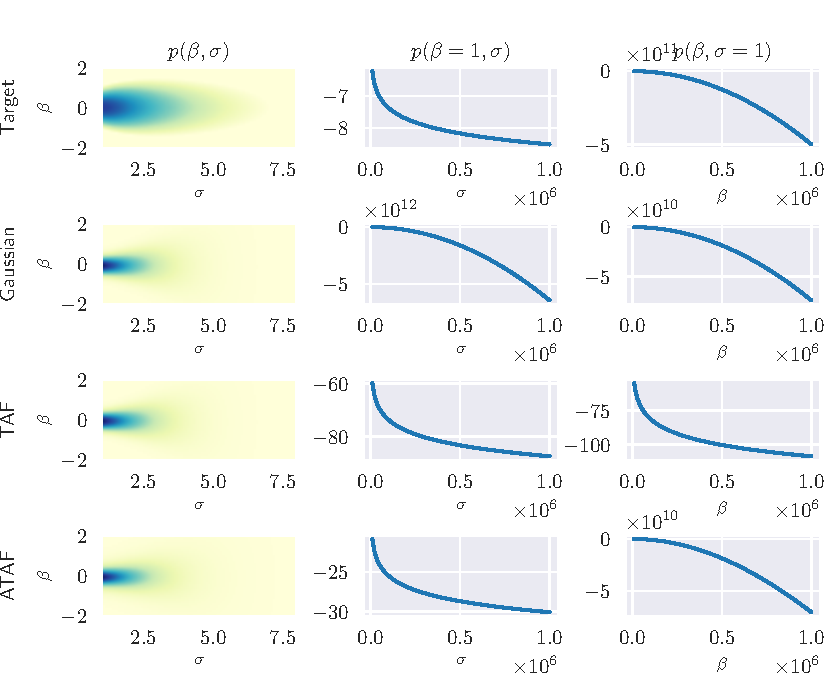
\includegraphics{../Figures/blr_aniso.pdf}
  \vspace{-0.3cm}
  \caption{
    Bayesian linear regression's tail-anisotropic posterior
    (top left) exhibits a fat-tailed conditional in $\sigma$ (as evidenced by
    the convex power-law decay in the top middle panel) and a Gaussian conditional in $\beta$ (concave graph in top right panel).
    While all methods appear to provide a good approximation of the bulk (left column),
    \Cref{prop:isotropic-pushforward} implies
    Gaussian (Gaussian, second row) or isotropic StudentT product (TAF, third row) base distributions
    yield Gaussian or power-law tails, respectively, for \emph{both} $\sigma$ and $\beta$.
    In contrast, ATAF (bottom row) illustrates \Cref{remark:anisotropic} by
    modeling simultaneously a power-law tail on $\sigma$ and Gaussian tail on $\beta$.
  }
  \label{fig:blr-anisotropic}
\end{figure*}

\begin{table*}[htbp]
  \centering
%   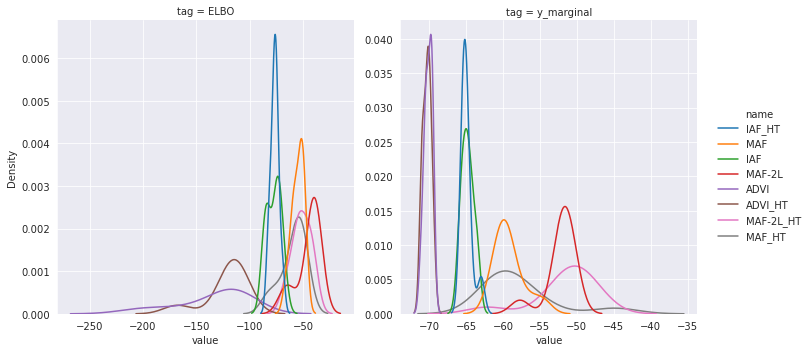
\includegraphics[width=1.0\textwidth]{../Figures/eight_schools.png}
    \begin{subfigure}[t]{0.49\textwidth}
        \centering
        \begin{tabular}{rcc}
            \toprule
                      & ELBO                & $\log p(y)$       \\
            \midrule
            ADVI      & $\mathbf{2873.90} \pm 6.95$    & $2969.73 \pm 1.73$ \\
            TAF       & $2839.64 \pm 9.10$    & $2973.85 \pm 0.87$ \\
            ATAF      & $2842.75 \pm 8.83$    & $\mathbf{2976.75} \pm 0.66$ \\
            \hline
            NUTS      & n/a                  & $3724.59 \pm 0.036$ \\
            \bottomrule
        \end{tabular}
        \caption{diamonds}
        \label{tab:diamonds}
    \end{subfigure}
    \begin{subfigure}[t]{0.49\textwidth}
        \centering
        \begin{tabular}{rcc}
            \toprule
                      & ELBO                & $\log p(y)$       \\
            \midrule
            ADVI      & $-72.13 \pm 6.89$    & $-53.25 \pm 3.44$ \\
            TAF       & $-64.64 \pm 4.88$    & $-52.51 \pm 4.41$ \\
            ATAF      & $\mathbf{-58.63} \pm 4.75$    & $\mathbf{-51.01} \pm 3.71$ \\
            \hline
            NUTS      & n/a                  & $-47.78 \pm 0.093$ \\
            \bottomrule
        \end{tabular}
        \caption{Eight schools}
        \label{tab:eight_schools}
    \end{subfigure}
    \vspace{-2mm}
        \caption{Monte-Carlo ELBO and importance weighted Monte-Carlo marginal likelihood
        $p(y) = \EE_{x \sim q_\theta} \frac{p(x,y)}{q_\theta(x)}$ (higher is better, $\pm$ standard errors)
        estimates from VI on real-world datasets.
        To understand the variational approximation gap, we include marginal likelihoods based on ``golden samples'' from \texttt{posteriordb} \citep{ghposteriordb} computed using No-U-Turn-Sampling (NUTS, \citet{hoffman2014no,carpenter2017stan}).
    }
  \label{fig:eight_schools}
  \vspace{-4mm}
\end{table*}


\begin{table*}[htbp]
    \centering
    \begin{tabular}{rcc}
        \toprule
                  & Fama-French 5 Industry Daily & CMS 2008-2010 DE-SynPUF       \\
        \midrule
        ADVI      & $-5.018 \pm 0.056$    & $-1.883 \pm 0.012$ \\
        TAF       & $-4.703 \pm 0.023$    & $-1.659 \pm 0.004$ \\
        ATAF      & $\mathbf{-4.699} \pm 0.024$    & $\mathbf{-1.603} \pm 0.034$ \\
        \bottomrule
    \end{tabular}
    \vspace{-2mm}
    \caption{
        Log-likelihoods (higher is better, $\pm$ standard errors) achieved on
        density modeling tasks involving financial returns \citep{fama2015five} and insurance claims \citep{cms} data. 
        \vspace{-5mm}
    }
    \label{tab:density-estimation}
\end{table*}



\subsection{Bayesian Linear Regression}

Consider one-dimensional Bayesian linear regression (BLR)
with conjugate priors, defined by priors and likelihood
\begin{gather*}
    \sigma^2 \sim \text{Inv-Gamma}(a_0, b_0)\\
    \beta \mid \sigma^2 \sim \cN(0, \sigma^2),\qquad
    y \mid X, \beta, \sigma \sim \cN(X \beta, \sigma^2) ,
\end{gather*}
where $a_0$, $b_0$ are hyperparameters and the task is to approximate the posterior
distribution $p(\beta,\sigma^2 \mid X, y)$. Owing to conjugacy,
the posterior distribution can be explicitly computed. Indeed, $p(\beta,\sigma^2 \mid X, y) = \rho(\sigma^2)\rho(\beta \mid \sigma)$ where $\rho(\beta \mid \sigma) = \cN(\Sigma_n(X^\top X \hat\beta), \sigma^2 \Sigma_n)$, $\Sigma_n = (X^\top X + \sigma^{-2})^{-1}$, $\hat\beta = (X^\top X)^{-1} X^\top y$, and
%\begin{align*}
    %p(\beta,\sigma^2 \mid X, y) &= \rho(\sigma^2) \rho(\beta \mid \sigma) \\
    \[
    \rho(\sigma^2) = \text{Inv-Gamma}\bigg(
    %\underbrace{a_0 + \frac{n}{2}}_{\eqqcolon a_n}, 
    a_0 + \frac{n}{2}, 
    b_0 + \frac{1}{2}(y^\top y - \mu_n^\top \Sigma_n \mu_n)\bigg). % \\
    \]
    %\rho(\beta \mid \sigma) &= \cN(\Sigma_n(X^\top X \hat\beta), \sigma^2 (X^\top X + \sigma^{-2} I)^{-1})
%\end{align*}
This calculation reveals that the posterior distribution is tail-anisotropic:
for fixed $c$ we have that $p(\sigma^2, \beta=c \mid X, y) \propto \rho(\sigma^2) \in \cL^1_{\alpha_n}$
as a function of $\sigma$ (with $\alpha_n$ a function of $n$)
and $p(\sigma^2=c, \beta \mid X, y) \propto \rho(\beta \mid c) \in \overline{\cE^2}$
as a function of $\beta$.
As a result of \Cref{prop:isotropic-pushforward}, we expect ADVI and TAF to erroneously impose
Gaussian and power-law tails respectively for both $\beta$ and $\sigma^2$ as neither method
can produce a tail-anisotropic pushforward. This intuition is confirmed in \Cref{fig:blr-anisotropic},
where we see that only ATAF is the only method capable of modeling the tail-anisotropy present in the data.

Conducting Bayesian linear regression is among the standard tasks requested of a probabilistic programming language, yet it still displays tail-anisotropy. To accurately capture large quantiles, this tail-anisotropy  should not be ignored, necessitating a method such as ATAF.

\subsection{Diamond Price Prediction Using Non-Conjugate Bayesian Regression}
\label{ssec:diamonds}

Without conjugacy, the BLR posterior is intractable and there is no reason \emph{a priori} to expect tail-anisotropy.
Regardless, this presents a realistic and practical scenario for evaluating ATAF's ability to improve VI.
For this experiment, we consider BLR on the \texttt{diamonds} dataset \citep{wickham2011ggplot2} included in
\texttt{posteriordb} \citep{ghposteriordb}.
This dataset contains a covariate matrix $X \in \RR^{5000 \times 24}$ consisting of $5000$
diamonds each with $24$ features as well as an outcome variable $y \in \RR^{5000}$ representing each diamond's price.
The probabilistic model for this inference task is specified in Stan code provided by \citet{ghposteriordb} and is reproduced here
for convenience:
\begin{gather*}
    \alpha \sim \text{StudentT}(\nu=3, \text{loc}=8, \text{scale}=10)\\
    \sigma \sim \text{HalfStudentT}(\nu=3, \text{loc}=0, \text{scale}=10)\\
    \beta \sim \cN(0, \mI_{24}),\qquad
    y \sim \cN(\alpha + X \beta, \sigma) .
\end{gather*}

For each VI method, we performed 100 trials each consisting of 5000 descent steps
on the Monte-Carlo ELBO estimated using 1000 samples and report the results in
\Cref{tab:diamonds}. We report both the final Monte-Carlo ELBO
as well as a Monte-Carlo importance-weighted approximation to
the log marginal likelihood $\log p(y) = \log \EE_{x \sim q_\theta} \frac{p(x,y)}{q_\theta(y)}$
both estimated using 1000 samples.

% \subsection{Bayesian Robust Linear Regression}

% $n = 100$, $d = 10$.

% $X_{ij} \simiid N(0,1)$ for $i \in [n]$, $j \in [d]$.

% $y_i \simiid \text{StudentT}(\text{loc}=X \beta, df=5)$

% Improper ``flat'' prior on $\beta$ to ensure heavy-tailed posterior.

% \begin{figure}[H]
%   \centering
%   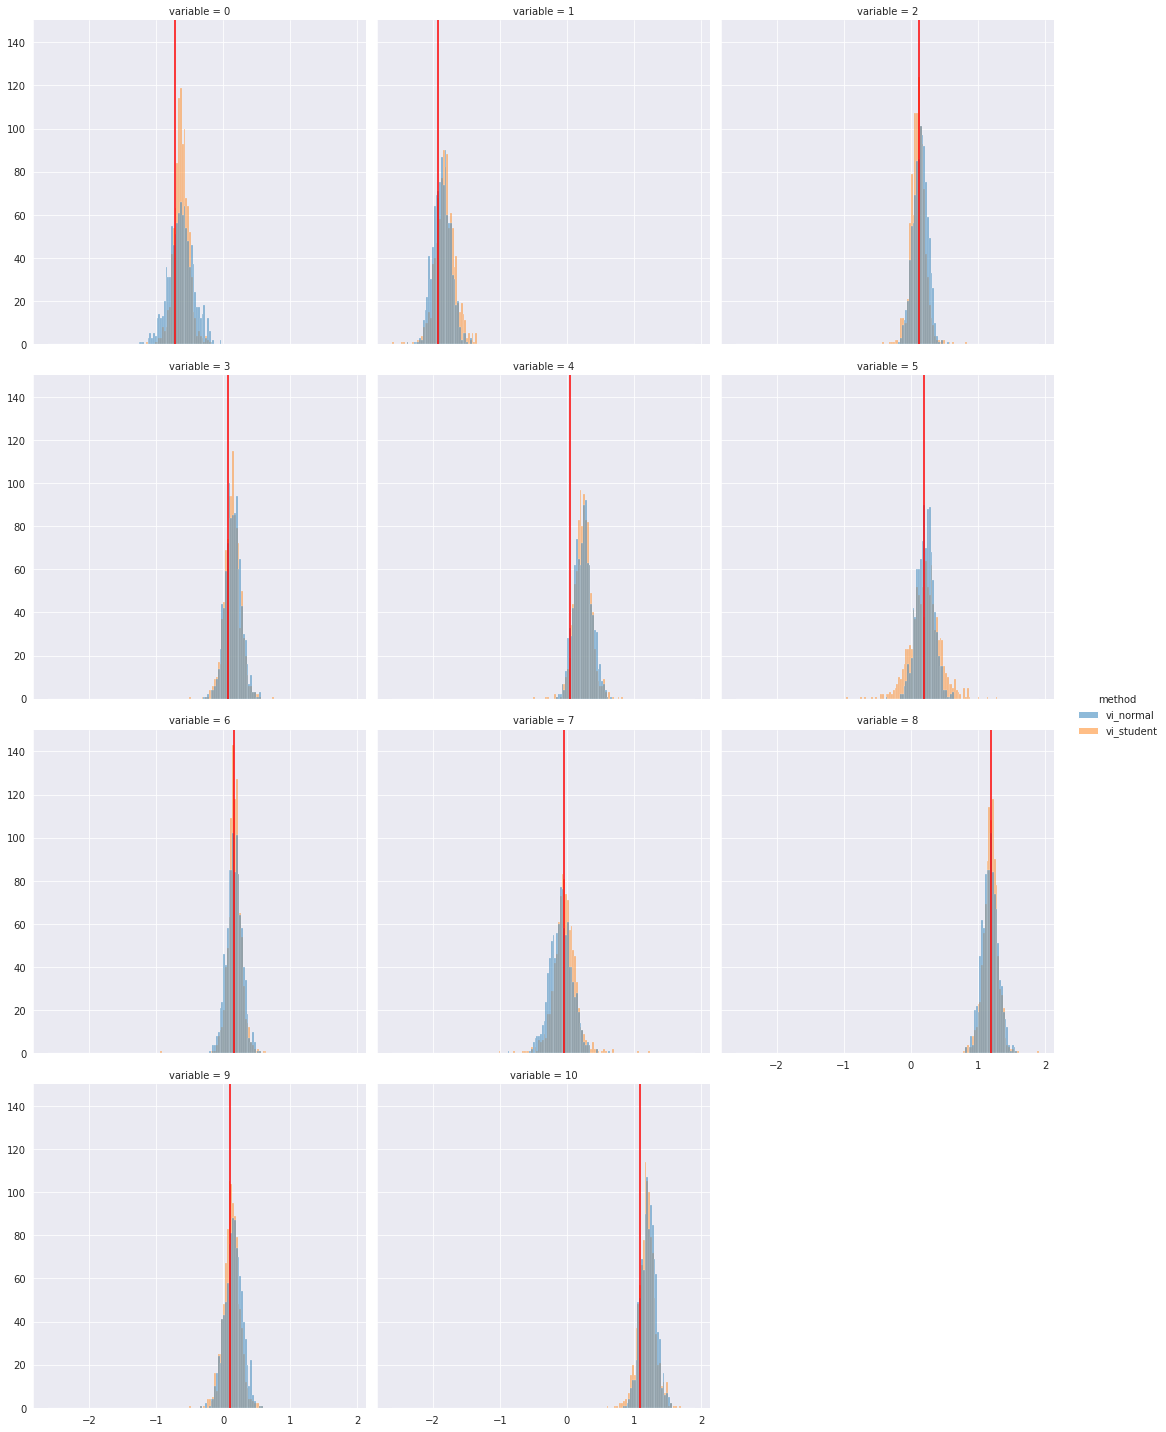
\includegraphics[width=0.9\textwidth]{../Figures/blr.png}
%   \caption{VI of Bayesian robust linear regression}
%   \label{fig:blr}
% \end{figure}

\subsection{Eight Schools SAT Score Modelling with Fat-tailed Scale Mixtures}
\label{ssec:eight_schools}

The eight-schools model \citep{rubin1981estimation,gelman2013bayesian} is a classical
Bayesian hierarchical model used originally to consider the relationship between standardized
test scores and coaching programs in place at eight schools.
A variation using half Cauchy non-informative priors \citep{gelman2006prior} provides
a real-world inference problem involving fat-tailed distributions, and is formally specified
by the probabilistic model
\begin{gather*}
    \tau \sim \text{HalfCauchy}(\text{loc}=0, \text{scale}=5)\\
    \mu \sim \cN(0, 5),\qquad
    \theta \sim \cN(\mu, \tau),\qquad
    y \sim \cN(\theta, \sigma) .
\end{gather*}
Given test scores and standard errors $\{(y_i, \sigma_i)\}_{i=1}^8$, we are interested in the
posterior distribution over treatment effects $\theta_1,\ldots,\theta_d$. The experimental
parameters are identical to \Cref{ssec:diamonds}, and results are reported in \Cref{tab:eight_schools}.


\subsection{Financial and Actuarial Applications}

To examine the advantage of tail-anisotropic modelling in practice, we considered two benchmark datasets from financial (daily log returns for five industry indices during 1926--2021 \citep{fama2015five}) and actuarial (per-patient inpatient and outpatient cumulative Medicare/Medicid (CMS) claims during 2008--2010 \citep{cms}) applications where practitioners actively seek to model fat-tails and account for black-swan events. Identical flow architectures and optimizers were used in both cases, with log-likelihoods presented in \Cref{tab:density-estimation}. Both datasets exhibited superior fits after allowing for heavier tails, with a further improved fit using ATAF for the CMS claims dataset. 
%Using identical flow architectures and optimizers, the log likelihoods in \Cref{tab:density-estimation} suggest that models permitting tail-anisotropy (ATAF) yield significantly superior fits.


% \feynman{TODO}

% \subsection{Bayesian regression analysis on diamonds}
% \feynman{Remove? These are taking too long and don't look good}

% \begin{table}[htbp]
%   \caption{Final ELBO and (MC estimate of) log marginal $\log P(y)$ after 10000 steps on \texttt{diamonds}}
%   \label{fig:blr_diamonds}
%   \centering
%   \begin{tabular}{rcc}
%     \toprule
%               & ELBO   & $\log P(y)$ \\
%     \midrule
%     ADVI      & -374.4 & -6912.0           \\
%     ADVI-HT   & -246.3 & -6876.6     \\
%     MAF       & -211.1 & -6894.8     \\
%     MAF-HT    & -208.5 & -7442.0     \\
%     MAF-2L    & -197.9 & -6532.4     \\
%     MAF-2L-HT & -191.9 & -6839.9     \\
%     MAF-3L    & -194.1 & -7027.3     \\
%     MAF-3L-HT & -209.8 & -7128.1     \\
%     \bottomrule
%   \end{tabular}
% \end{table}


% \feynman{
%   % \subsection{Importance weights}

%   When the importance sampling density is more peaked than the target density.

%   \cite{wang2018variational} example 3.1: Let $p = N(0, \sigma_p^2)$, $q = N(0, \sigma_q^2)$,
%   and for $x \sim q$ let $w(x) = \frac{p(x)}{q(x)}$. If $\sigma_p > \sigma_q$,
%   then $w$ has tail index $\frac{\sigma_p^2}{\sigma_p^2 - \sigma_q^2}$.
%   Otherwise, $w$ is not fat-tailed.
% }

%\section{Related Work}



\section{Conclusion}
\label{sec:conclusion}

In this work, we have sharpened existing theory for approximating fat-tailed distributions with normalizing flows, and we formalized tail-(an)isotropy through a direction-dependent tail parameter. With this, we have shown that many prior flow-based methods are inherently limited by tail-isotropy. With this in mind, we proposed a simple flow-based method capable of modeling tail-anisotropic targets.
As we have seen, anisotropic FTVI is already applicable in fairly elementary examples such as Bayesian linear regression;
and ATAFs provide one of the first methods for using the representational capacity of flow-based methods,
while simultaneously producing tail-anisotropic distributions. A number of open problems still remain, including the study of other parameterizations of the tail behaviour of the base distribution. Even so, going forward, it seems prudent that density estimators, especially those used in black-box settings, consider accounting for tail-anisotropy using a method such as~ATAF.% expect the scientific impact of ATAFs to be
%fairly easily realized, as it can be applied wherever a parametric density estimator is used.
%While we do not expect ATAF to directly have any negative societal impacts,
%its broad applicability as a parametric density estimator which accommodates fat-tails means that it may be
%used to improve applications which do cause negative societal impact.

% VI is important, FTVI is very important, ADVI did a good job with FTVI, we do a great job with FTVI, and you the reader should follow up on us and do FTVI.

\paragraph{Acknowledgements}
L.H. and M.M's contributions were supported in part by DARPA, NSF, and ONR.
F.L.’s research while at the University of California, Berkeley was supported in part by a GFSD fellowship.


\bibliography{refs_ftvi}
\bibliographystyle{icml2022}

%%%%%%%%%%%%%%%%%%%%%%%%%%%%%%%%%%%%%%%%%%%%%%%%%%%%%%%%%%%%
% \section*{Checklist}

% %%% BEGIN INSTRUCTIONS %%%
% % The checklist follows the references.  Please
% % read the checklist guidelines carefully for information on how to answer these
% % questions.  For each question, change the default \answerTODO{} to \answerYes{},
% % \answerNo{}, or \answerNA{}.  You are strongly encouraged to include a {\bf
% %     justification to your answer}, either by referencing the appropriate section of
% % your paper or providing a brief inline description.  For example:
% % \begin{itemize}
% %   \item Did you include the license to the code and datasets? \answerYes{See Section~\ref{gen_inst}.}
% %   \item Did you include the license to the code and datasets? \answerNo{The code and the data are proprietary.}
% %   \item Did you include the license to the code and datasets? \answerNA{}
% % \end{itemize}
% % Please do not modify the questions and only use the provided macros for your
% % answers.  Note that the Checklist section does not count towards the page
% % limit.  In your paper, please delete this instructions block and only keep the
% % Checklist section heading above along with the questions/answers below.
% %%% END INSTRUCTIONS %%%

% \begin{enumerate}

%   \item For all authors...
%         \begin{enumerate}
%           \item Do the main claims made in the abstract and introduction accurately reflect the paper's contributions and scope?
%                 \answerYes{}
%           \item Did you describe the limitations of your work?
%                 \answerYes{See \Cref{ssec:limitations}}
%           \item Did you discuss any potential negative societal impacts of your work?
%                 \answerYes{See \Cref{sec:conclusion}}
%           \item Have you read the ethics review guidelines and ensured that your paper conforms to them?
%                 \answerYes{}
%         \end{enumerate}

%   \item If you are including theoretical results...
%         \begin{enumerate}
%           \item Did you state the full set of assumptions of all theoretical results?
%                 \answerYes{}
%           \item Did you include complete proofs of all theoretical results?
%                 \answerYes{Deferred to \Cref{sec:proofs}}
%         \end{enumerate}

%   \item If you ran experiments...
%         \begin{enumerate}
%           \item Did you include the code, data, and instructions needed to reproduce the main experimental results (either in the supplemental material or as a URL)?
%                 \answerYes{See \Cref{sec:experiments}}
%           \item Did you specify all the training details (e.g., data splits, hyperparameters, how they were chosen)?
%                 \answerYes{See \Cref{sec:experiments}, \Cref{sec:additional-exp-details}, and open-sourced code}
%           \item Did you report error bars (e.g., with respect to the random seed after running experiments multiple times)?
%                 \answerYes{Tables/figures report standard errors}
%           \item Did you include the total amount of compute and the type of resources used (e.g., type of GPUs, internal cluster, or cloud provider)?
%                 \answerYes{See \Cref{sec:additional-exp-details}}
%         \end{enumerate}

%   \item If you are using existing assets (e.g., code, data, models) or curating/releasing new assets...
%         \begin{enumerate}
%           \item If your work uses existing assets, did you cite the creators?
%                 \answerYes{}
%           \item Did you mention the license of the assets?
%                 \answerYes{See \texttt{LICENSE} and \texttt{README.md} file on Github repository.}
%           \item Did you include any new assets either in the supplemental material or as a URL?
%                 \answerYes{Experiments use newly developed code within \texttt{beanmachine} which is released in \Cref{sec:experiments}.}
%           \item Did you discuss whether and how consent was obtained from people whose data you're using/curating?
%                 \answerNo{Datasets used are either synthetic or released as part of MIT/BSD-3 licensed code.}
%           \item Did you discuss whether the data you are using/curating contains personally identifiable information or offensive content?
%                 \answerNo{We did not screen datasets for PII / offensive content. All experiments perform probabilistic modeling on top of
%                 existing data, so we do not expect any PII / offensive content to appear in the body of the paper. Please notify us if something
%                 could potentially make a reader uncomfortable and we will be happy to fix it!
%                 }
%         \end{enumerate}

%   \item If you used crowdsourcing or conducted research with human subjects...
%         \begin{enumerate}
%           \item Did you include the full text of instructions given to participants and screenshots, if applicable?
%                 \answerNA{}
%           \item Did you describe any potential participant risks, with links to Institutional Review Board (IRB) approvals, if applicable?
%                 \answerNA{}
%           \item Did you include the estimated hourly wage paid to participants and the total amount spent on participant compensation?
%                 \answerNA{}
%         \end{enumerate}

% \end{enumerate}

%%%%%%%%%%%%%%%%%%%%%%%%%%%%%%%%%%%%%%%%%%%%%%%%%%%%%%%%%%%%
\newpage
\appendix
\onecolumn

\section{Experiments Performing VI Against a Fat-tailed Cauchy Target}
\label{sec:cauchy_normal_student}
The motivation for the fat-tailed variational families used in TAF/ATAF
is easily illustrated on a toy example consisting of $X \sim \text{Cauchy}(x_0 = 0, \gamma = 1) \in \cL^1_1$.
As seen in \Cref{fig:cauchy_normal_student}, while ADVI with normalizing flows \citep{kingma2016improved,webb2019improving}
appears to provide a reasonable fit to the bulk of the target distribution (left panel), the improper
imposition of sub-Gaussian tails results in an exponentially bad tail approximation (middle panel).
As a result, samples drawn from the variational approximation fail a Kolmogorov-Smirnov goodness-of-fit
test against the true target distribution much more often (right panel, smaller $p$-values imply more rejections)
than a variational approximation which permits fat-tails. This example is a special case of \Cref{thm:distn_class_closed}.

\begin{figure*}[htbp]
  \centering
  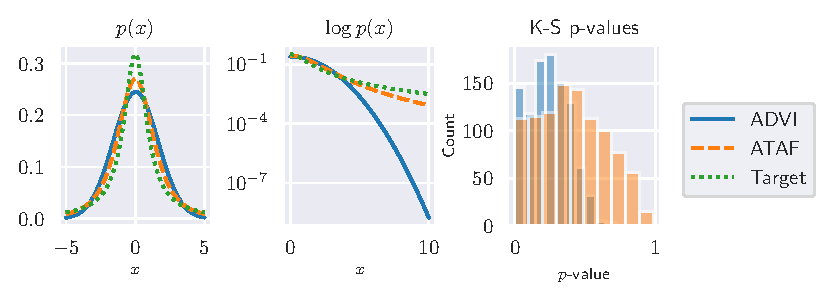
\includegraphics{../Figures/fat_tail_ks.pdf}
  \vspace{-6mm}
  \caption{
    When performing FTVI to approximate a $X \sim \text{Cauchy}(x_0 = 0, \gamma = 1)$ target (left panel, green dotted line),
    the use of a Gaussian variational family (ADVI, solid blue line) can incur
    exponentially bad tail approximations (middle panel) compared to
    methods such as ATAF which permit heavier tails (orange dashed line).
    As a consequence, ADVI samples (blue, right panel) are rejected by
    the Kolmogorov-Smirnov test more often than ATAF samples (orange, right panel).
    % \michael{Why does (b) look so good; are the tails really perfect, of if we went out to 15 or 30 on the X axis.  It might be good to show ATAF is much better but still not perfect.  Also, what is the X axis on each figure.  }
  }
  \label{fig:cauchy_normal_student}
\end{figure*}

\section{Proofs of Our Main Theoretical Results}
\label{sec:proofs}

\begin{proof}[Proof of \Cref{thm:distn_class_closed}]
  \label{proof:distn_class_closed}
  Let $X$ be a random variable from either $\cE_\alpha^p$
  or $\cL_\alpha^p$.
  Its concentration function
  (Equation 1.6 \citet{ledoux2001concentration}
  is given by
  \[
    \alpha_X(r)
    \coloneqq \sup \{ \mu\{x : d(x,A) \geq r\}; A \subset \text{supp}~X, \mu(A) \geq 1/2\}
    = \PP(\lvert X - m_X \rvert \geq r) .
  \]
  Under Assumption 1, $f_\theta$ is Lipschitz (say with Lipschitz
  constant $L$) so by Proposition 1.3 of \citet{ledoux2001concentration},
  \[
    \PP(\lvert f_\theta(X) - m_{f_\theta(X)}\rvert \geq r)
    \leq 2 \alpha_X(r/L)
    = \cO(\alpha_X(r/L)),
  \]
  where $m_{f_\theta(X)}$ is a median of $f_\theta(X)$.
  Furthermore, by the triangle inequality
  \begin{align}
    \PP(\lvert f_\theta(X) \rvert \geq r)
    &= \PP(\lvert f_\theta(X) - m_{f_\theta(X)} + m_{f_\theta(X)} \rvert \geq r) \nonumber\\
    &\leq \PP(\lvert f_\theta(X) - m_{f_\theta(X)}\rvert \geq r - \lvert m_{f_\theta(X)}\rvert ) \nonumber\\
    &= \cO(\PP(\lvert f_\theta(X) - m_{f_\theta(X)}\rvert \geq r)) \nonumber\\
    &= \cO(\alpha_X(r/L)) ,
    \label{eq:pushforward-conc-fn}
  \end{align}
  where the asymptotic equivalence holds because $\lvert m_{f_\theta(X)} \rvert$ is independent of $r$.
  When $X \in \cE_\alpha^p$, \Cref{eq:pushforward-conc-fn} implies
  \[
    \PP(\lvert f_\theta(X) \rvert \geq r)
    = \cO(e^{-\frac{\alpha}{L} r^p}) \implies f_\theta(X) \in \overline{\cE}_{\alpha/L}^p,
  \]
  from whence we find that the Lipschitz transform of exponential-type
  tails continues to possess exponential-type tails with the same
  class index $p$, although the tail parameter may have changed. Hence,
  $\overline{\cE^p}$ is closed under Lipschitz maps for each $p \in \RR_{>0}$.
  On the other hand, when $X \in \cL_\alpha^p$, \Cref{eq:pushforward-conc-fn} also implies that
  \begin{align*}
    \PP(\lvert f_\theta(X) \rvert \geq r)
    &= \cO(e^{-\alpha (\log (r/L))^p})
    % &= \cO(e^{-\alpha (\log r)^p} e^{-\alpha (-\log L)^p}) \\
    = \cO(e^{-\alpha (\log r)^p}),
  \end{align*}
  and therefore, $f_\theta(X) \in \overline{\cL_\alpha^p}$.
  Unlike exponential-type tails, Lipschitz transforms of
  logarithmic-type tails not only remain logarithmic, but
  their tails decay no slower than a logarithmic-type tail
  of the same class index with the \emph{same} tail parameter $\alpha$.
  This upper bound suffices to show closure under Lipschitz maps for the
  ascending family $\overline{\cL_\alpha^p}$.
\end{proof}

\begin{proof}[Proof of \Cref{corr:heavy_to_light}]
    Let $f_\theta$ be as before with the additional assumptions.
    Since $f_\theta$ is a smooth continuous bijection, it is a diffeomorphism.
    Furthermore, by assumption $f_\theta$ has invertible Jacobian on the closure of its
    domain hence $\sup_{x \in \text{dom}~f_\theta} \lvert (f_\theta)'(x) \rvert \geq M > 0$.
    By the inverse function theorem, $(f_\theta)^{-1}$ exists and is
    a diffeomorphism with
    \[
    \frac{d}{dx}(f_\theta)^{-1}(x) = \frac{1}{(f_\theta)'((f_\theta)^{-1}(x))} \leq \frac{1}{M} .
    \]
    Therefore, $(f_\theta)^{-1}$ is $M^{-1}$-Lipschitz and we may apply
    \Cref{thm:distn_class_closed} to conclude the desired result.
    %\footnote{\url{https://math.stackexchange.com/questions/394908/diffeomorphism-from-inverse-function-theorem}}
\end{proof}

\begin{proof}[Proof of \Cref{corr:closure_polynomials}]
  Let $X \in \cE^p_\alpha$.
  By considering sufficiently large $X$ such that leading powers dominate, it suffices to consider monomials $Y = X^k$.
  Notice $\PP(Y \geq x) = \PP(X \geq x^{1/k}) = \Theta(e^{-\alpha x^{p/k}})$, and so
  $Y \in \cE^{p/k}_\alpha$. The result follows by disjointness of $\mathcal{E}$ and $\mathcal{L}$. 
\end{proof}

\begin{lemma}
    \label[lemma]{lem:sum-rule}
    Suppose $X \in \cL^1_\alpha$ and $Y \in \cL^1_\beta$.
    Then $X + Y \in \cL^1_{\min\{\alpha,\beta\}}$.
\end{lemma}

\begin{proof}
First, let $\gamma=\min\{\alpha,\beta\}$. It will suffice to show that (I) $\mathbb{P}(|X+Y|\geq r)=\mathcal{O}(r^{-\gamma})$, and (II) $\mathbb{P}(|X+Y|\geq r)\geq\Theta(r^{-\gamma})$. Since $(X,Y)\mapsto|X+Y|$ is a 1-Lipschitz function on $\mathbb{R}^{2}$ and $\mathbb{P}(|X|\geq r)+\mathbb{P}(|Y|\geq r)=\mathcal{O}(r^{-\gamma})$, (I) follows directly from the hypotheses and Proposition 1.11 of \citet{ledoux2001concentration}. To show (II), note that for any $M>0$, conditioning on the event $|Y|\leq M$,\[
\mathbb{P}\left(\left|X\right|+|Y|\geq r\,\vert\,|Y|\leq M\right)\geq\mathbb{P}\left(\left|X\right|\geq r-M\right).
\]
Therefore, by taking $M$ to be sufficiently large so that $\mathbb{P}(|Y|\leq M)\geq\frac{1}{2}$,
\begin{align*}
\mathbb{P}\left(|X+Y|\geq r\right)&\geq\mathbb{P}\left(|X|+|Y|\geq r\right)\\
&\geq\mathbb{P}\left(\left|X\right|+|Y|\geq r\,\vert\,|Y|\leq M\right)\mathbb{P}\left(\left|Y\right|\leq M\right)\\
&\geq\frac{1}{2}\mathbb{P}\left(\left|X\right|\geq r-M\right)=\Theta(r^{-\alpha}).
\end{align*}
The same process with $X$ and $Y$ reversed implies $\mathbb{P}(|X+Y|\geq r)\geq\Theta(r^{-\beta})$ as well. Both (II) and the claim follow.
\end{proof}

To show Proposition \ref{prop:isotropic-pushforward}, we will require a few extra assumptions to rule out pathological cases. The full content of Proposition \ref{prop:isotropic-pushforward} is contained in the following theorem.

\begin{theorem}
Suppose there exists $\nu > 0$ such that $C:\mathcal{S}^{d-1}\to(0,\infty)$ satisfies $C(v) \coloneqq \lim_{x \to \infty}x^{\nu}\mathbb{P}(|\langle v, X\rangle| > x)$ for all $v \in \mathcal{S}^{d-1}$. If $\nu$ is not an integer and $f$ is a bilipschitz function,
%such that $f(X)/\|f(X)\|$ has full support on $\mathcal{S}^{d-1}$
then $f(X)$ is tail-isotropic with tail index $\nu$. 
\end{theorem}
\begin{proof}
Since $x \mapsto \langle v, f(x)\rangle$ is Lipschitz continuous for any $v \in \mathcal{S}^{d-1}$, Theorem \ref{thm:distn_class_closed} implies $\langle v, f(X)\rangle \in \overline{\mathcal{L}_{\nu}^{1}}$. Let $\theta \in (0,\pi/2)$ (say, $\theta = \pi / 4$), and let $S_v = \{x\, : \, \cos^{-1}(\langle x/\|x\|, v\rangle)\leq\theta\}$ for each $v \in \mathcal{S}^{d-1}$. Then
\[
H_v \coloneqq \{x\,:\,\langle v, x \rangle > 1\} \supset \{x\,:\,\|x\| > (1-\cos\theta)^{-1}\} \cap S_v.
\]
From Theorem C.2.1 of \citet{buraczewski2016stochastic}, since $\nu \not \in \mathbb{Z}$, there exists a non-zero measure $\mu$ such that
\[
\mu(E) = \lim_{x \to \infty} \frac{\mathbb{P}(x^{-1}X \in E)}{\mathbb{P}(\|X\| > x)},
\]
for any Borel set $E$. Consequently, $\mu$ is regularly varying, and so 
by the spectral representation of regularly varying random vectors (see p. 281 \citet{buraczewski2016stochastic}), there exists a measure $P$ such that
\[
\lim_{x \to \infty}\frac{\mathbb{P}(\|X\|>tx, X/\|X\| \in E)}{\mathbb{P}(\|X\| > x)} = t^{-\nu} P(E),
\]
for any Borel set $E$ on $\mathcal{S}^{d-1}$ and any $t > 0$. Letting $F_v = \{y / \|y\|\,:\, f(y) \in S_v\} \subset \mathcal{S}^{d-1}$ (noting that $P(F_v) > 0$ by assumption), since $m\|x - y\| \leq \|f(x) - f(y)\| \leq M\|x - y\|$ for all $x,y$,
\begin{align*}
\liminf_{x \to \infty}
\frac{\mathbb{P}(f(X) \in x H_v)}{\mathbb{P}(\|f(X)\| > x)} 
&\geq \liminf_{x \to \infty}\frac{\mathbb{P}(\|f(X)\| > x(1-\cos\theta)^{-1}, f(X) \in S_v)}{\mathbb{P}(\|f(X)\| > x)} \\
&\geq \liminf_{x \to \infty}\frac{\mathbb{P}(\|X\| > x(m(1-\cos\theta))^{-1}, X/\|X\| \in F_v)}{\|X\| > x / M} \\
&\geq P(F_v) \left(\frac{M}{m(1-\cos\theta)}\right)^{-\nu} > 0,
yaB\end{align*}
where $P(F_v) > 0$ follows from the bilipschitz condition for $f$. Therefore, we have shown that $\mathbb{P}(\langle v, f(X)\rangle > x) = \Theta(\mathbb{P}(\|f(X)\| > x))$ for every $v \in \mathcal{S}^{d-1}$.
Since $\mathbb{P}(\|f(X)\| > x)$ obeys a power law with exponent $\nu$ by Corollary \ref{corr:heavy_to_light}, $f(X)$ is tail-isotropic with exponent $\nu$.
\end{proof}

%\begin{proof}[Proof of \Cref{prop:isotropic-pushforward}]
%  Since $f_\theta$ satisfies \cref{assump:lipschitz}, we have $\max(\|f_\theta\|_{\text{Lip}},\|f_\theta^{-1}\|_{\text{Lip}} \leq L < \infty$

%   Fix $z \in \cS^{d-1}$.
%   Note tail parameters are invariant under scalar multiplication as a consequence of
%   asymptotic notation, so combined with repeated applications of \Cref{lem:sum-rule} we
%   have that the linear combination $\braket{f_\theta(X), z}$
%   of $\{f_\theta(X)_i\}_{i \in [d]}$ is tail-isotropic provided
%   every $f_\theta(X)_i \in \cL_\nu^1$.
%   Let $i \in [d]$ be arbitrary.
%   Notice that the projection map $\pi_i = x \mapsto x_i$
%   is $1$-Lipschitz hence $\pi_i \circ f_\theta = x \mapsto f_\theta(x)_i$
%   is $L$-Lipschitz. In particular, $g_{x_{-i}} = x_i \mapsto (\pi \circ_i f_\theta)(x_{-i}, x_i)$ is $L$-Lipschitz for every $x_{-i} \in \mathbb{R}^{d-1}$.
  
%   Consider the $d$ times iterated conditional expectation
%   \begin{align*}
%       \mathbb{P}[f_\theta(X)_i \geq t]
%       &= \EE[\EE[\cdots\EE[1(f(X)_i \geq t) \mid X_1, \ldots, X_{i-1},X_{i+1},\ldots,X_d] \cdots \mid X_1 ]] \\
%       &= \EE[\EE[\cdots\mathbb{P}[g_{X_{-i}}(X_i) \geq t \mid X_{-i} ] \cdots \mid X_1 ]]
%   \end{align*}
%   Since $X \sim \mu$ is $\nu$-isotropic, we have that
%   $X_i = \braket{X, e_i} \in \cL_\nu^1$.
%   \feynman{To apply \cref{corr:heavy_to_light}, we need $x_i \mapsto f(x_{-i}, x_i)_i$ to be bi-Lipschitz for every $i \in [d]$ i.e. separately bilipschitz, see component Lipschitz constants in \url{http://www.optimization-online.org/DB_FILE/2014/12/4679.pdf}}
%\end{proof}


\section{Example of Non-existence of Tail Parameter Due to Oscillations}
\label{eg:spiral}

Consider $\text{StudentT}(\nu=1) \otimes \text{StudentT}(\nu=2)$ and ``spin'' it
using the radial transformation $(r,\theta) \mapsto (r,r+\theta)$ (\Cref{fig:spiral}). Due to
oscillations, $\alpha_X(v)$ is not well defined for all $v \in \cS^{1}$.


\begin{figure*}[htbp]
    \centering
    \vspace{-.5in}
    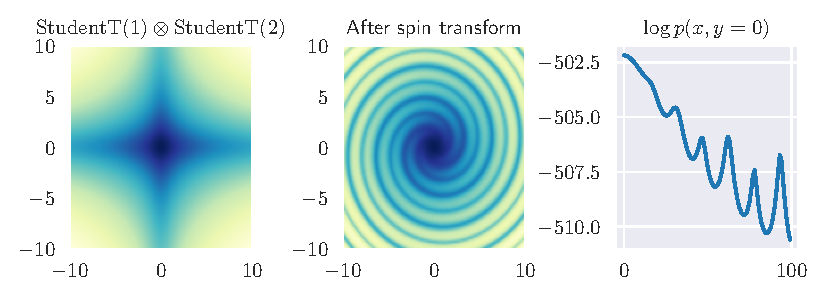
\includegraphics[scale=0.8]{Figures/spiral.pdf}
    % 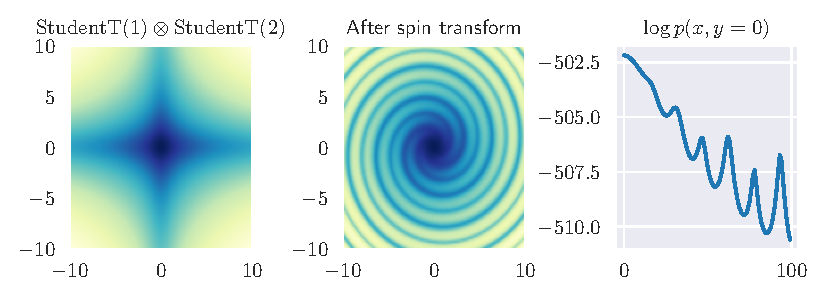
\includegraphics[trim={0 0 9cm 0},clip]{Figures/spiral.pdf}\\
    % 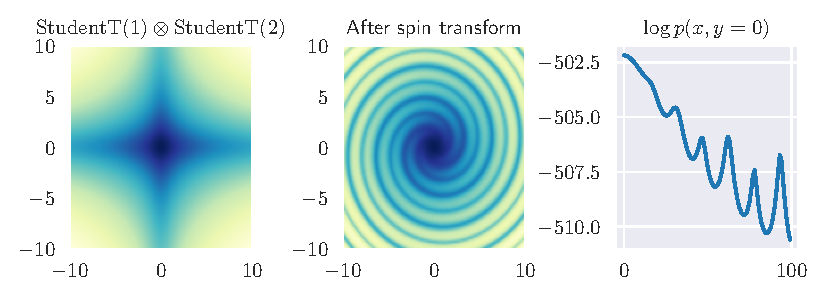
\includegraphics[trim={5cm 0 4.9cm 0},clip]{Figures/spiral.pdf}\\
    % 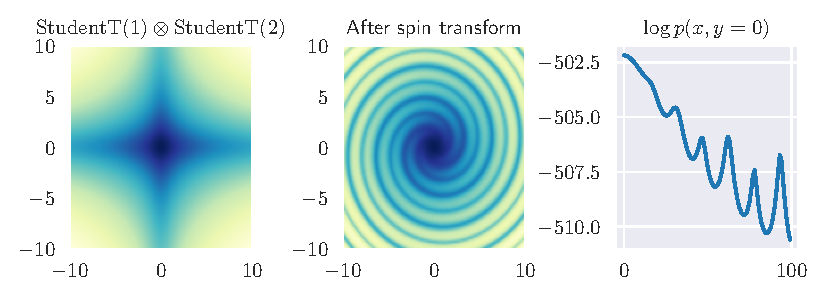
\includegraphics[trim={9.3cm 0 0cm 0},clip]{Figures/spiral.pdf}\\
    \caption{Taking a tail-anisotropic distribution (left) and ``spinning'' it (middle) results in
        one-dimensional projections which oscillate between tail parameters (as seen in
        $\log p(\braket{X,e_0})$ in right panel) and result in an ill-defined
        direction-dependent tail parameter function $\alpha_X(\cdot)$ due to a
        divergent limit.
    }
    \label{fig:spiral}
\end{figure*}


\section{Normal-normal Conjugate Model}
\label{sec:normal-normal-location-mixture}

We consider a Normal-Normal conjugate inference problem where the posterior
is known to be a Normal distribution as well. Here, we aim to show that ATAF
performs no worse than ADVI because $\text{StudentT}(\nu) \to N(0, 1)$ as $\nu \to \infty$.
\Cref{fig:normal_normal} shows the resulting density approximation, which can
be seen to be reasonable for both a Normal base distribution (the ``correct'' one)
and a StudentT base distribution. This suggests that mis-specification (i.e., heavier
tails in the base distribution than the target) may not be too problematic.

\begin{figure}[H]
  \centering
  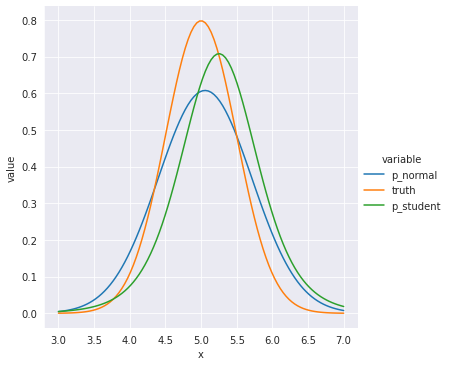
\includegraphics[width=0.6\textwidth]{../Figures/normal_normal_posterior.png}
  \caption{Variational inference against a light tailed Normal posterior. Both light and heavy tail
  variational families yield similar results.}
  \label{fig:normal_normal}
\end{figure}


\section{Additional Details For Experiments}
\label{sec:additional-exp-details}

All experiments were performed on an Intel i8700K with 32GB RAM and a NVIDIA GTX 1080
running PyTorch 1.9.0 / Python 3.8.5 / CUDA 11.2 / Ubuntu Linux 20.04 via Windows Subsystem for Linux.
For all flow-transforms $\Phi_{\text{Flow}}$, we used inverse autoregressive flows \citep{kingma2016improved} with a
dense autoregressive conditioner consisting of two layers of either 32 or 256 hidden units depending on problem (see code for details) and
ELU activation functions.
As described in \citet{jaini2020tails}, TAF is trained by including $\nu$ within the Adam optimizer alongside other flow parameters. For ATAF, we include all $\nu_i$ within the optimizer.
Models were trained using the Adam optimizer with $10^{-3}$ learning rate
for 10000 iterations, which we found empirically in all our experiments to result in negligible change in ELBO
at the end of training.

For \cref{tab:diamonds} and \cref{tab:eight_schools}, the flow transform $\Phi_{\text{Flow}}$ used for ADVI, TAF, and ATAF
is comprised of two hidden layers of 32 units each. NUTS uses no such flow transform. Variational parameters for each normalizing flow were initialized
using \texttt{torch}'s default Kaiming initialization \citep{he2015delving} Additionally, the tail parameters $\nu_i$
used in ATAF were initialized to all be equal to the tail parameters learned from training TAF. We empkkirically observed
this resulted in more stable results (less variation in ELBO / $\log p(y)$ across trials), which may be due to
the absence of outliers when using a Gaussian base distribution resulting in more stable ELBO gradients. This suggests
other techniques for handling outliers such as winsorization may also be helpful, and we leave further investigation
for future work.


For \cref{fig:blr-anisotropic}, the closed-form posterior was computed over a finite element grid to produce
the ``Target'' row. A similar progressive training scheme used for \cref{tab:diamonds} was also used here, with
the TAF flow transform $\Phi_{\text{Flow}}$ initialized from the result of ADVI and ATAF additionally initialized
all tail parameters $\nu_i$ based on the final shared tail parameter obtained from TAF training. Tails are computed
along the $\beta = 1$ or $\sigma = 1$ axes because the posterior is identically zero for $\sigma = 0$, hence it reveals
no information about the tails.

% \section{Electronic Submission}
% \label{submission}

% Submission to ICML 2022 will be entirely electronic, via a web site
% (not email). Information about the submission process and \LaTeX\ templates
% are available on the conference web site at:
% \begin{center}
% \textbf{\texttt{http://icml.cc/}}
% \end{center}

% The guidelines below will be enforced for initial submissions and
% camera-ready copies. Here is a brief summary:
% \begin{itemize}
% \item Submissions must be in PDF\@. 
% \item \textbf{New to this year}: If your paper has appendices, submit the appendix together with the main body and the references \textbf{as a single file}. Reviewers will not look for appendices as a separate PDF file. So if you submit such an extra file, reviewers will very likely miss it.
% \item Page limit: The main body of the paper has to be fitted to 8 pages, excluding references and appendices; the space for the latter two is not limited. For the final version of the paper, authors can add one extra page to the main body.
% \item \textbf{Do not include author information or acknowledgements} in your
%     initial submission.
% \item Your paper should be in \textbf{10 point Times font}.
% \item Make sure your PDF file only uses Type-1 fonts.
% \item Place figure captions \emph{under} the figure (and omit titles from inside
%     the graphic file itself). Place table captions \emph{over} the table.
% \item References must include page numbers whenever possible and be as complete
%     as possible. Place multiple citations in chronological order.
% \item Do not alter the style template; in particular, do not compress the paper
%     format by reducing the vertical spaces.
% \item Keep your abstract brief and self-contained, one paragraph and roughly
%     4--6 sentences. Gross violations will require correction at the
%     camera-ready phase. The title should have content words capitalized.
% \end{itemize}

% \subsection{Submitting Papers}

% \textbf{Paper Deadline:} The deadline for paper submission that is
% advertised on the conference website is strict. If your full,
% anonymized, submission does not reach us on time, it will not be
% considered for publication. 

% \textbf{Anonymous Submission:} ICML uses double-blind review: no identifying
% author information may appear on the title page or in the paper
% itself. \cref{author info} gives further details.

% \textbf{Simultaneous Submission:} ICML will not accept any paper which,
% at the time of submission, is under review for another conference or
% has already been published. This policy also applies to papers that
% overlap substantially in technical content with conference papers
% under review or previously published. ICML submissions must not be
% submitted to other conferences and journals during ICML's review
% period.
% %Authors may submit to ICML substantially different versions of journal papers
% %that are currently under review by the journal, but not yet accepted
% %at the time of submission.
% Informal publications, such as technical
% reports or papers in workshop proceedings which do not appear in
% print, do not fall under these restrictions.

% \medskip

% Authors must provide their manuscripts in \textbf{PDF} format.
% Furthermore, please make sure that files contain only embedded Type-1 fonts
% (e.g.,~using the program \texttt{pdffonts} in linux or using
% File/DocumentProperties/Fonts in Acrobat). Other fonts (like Type-3)
% might come from graphics files imported into the document.

% Authors using \textbf{Word} must convert their document to PDF\@. Most
% of the latest versions of Word have the facility to do this
% automatically. Submissions will not be accepted in Word format or any
% format other than PDF\@. Really. We're not joking. Don't send Word.

% Those who use \textbf{\LaTeX} should avoid including Type-3 fonts.
% Those using \texttt{latex} and \texttt{dvips} may need the following
% two commands:

% {\footnotesize
% \begin{verbatim}
% dvips -Ppdf -tletter -G0 -o paper.ps paper.dvi
% ps2pdf paper.ps
% \end{verbatim}}
% It is a zero following the ``-G'', which tells dvips to use
% the config.pdf file. Newer \TeX\ distributions don't always need this
% option.

% Using \texttt{pdflatex} rather than \texttt{latex}, often gives better
% results. This program avoids the Type-3 font problem, and supports more
% advanced features in the \texttt{microtype} package.

% \textbf{Graphics files} should be a reasonable size, and included from
% an appropriate format. Use vector formats (.eps/.pdf) for plots,
% lossless bitmap formats (.png) for raster graphics with sharp lines, and
% jpeg for photo-like images.

% The style file uses the \texttt{hyperref} package to make clickable
% links in documents. If this causes problems for you, add
% \texttt{nohyperref} as one of the options to the \texttt{icml2022}
% usepackage statement.


% \subsection{Submitting Final Camera-Ready Copy}

% The final versions of papers accepted for publication should follow the
% same format and naming convention as initial submissions, except that
% author information (names and affiliations) should be given. See
% \cref{final author} for formatting instructions.

% The footnote, ``Preliminary work. Under review by the International
% Conference on Machine Learning (ICML). Do not distribute.'' must be
% modified to ``\textit{Proceedings of the
% $\mathit{39}^{th}$ International Conference on Machine Learning},
% Baltimore, Maryland, USA, PMLR 162, 2022.
% Copyright 2022 by the author(s).''

% For those using the \textbf{\LaTeX} style file, this change (and others) is
% handled automatically by simply changing
% $\mathtt{\backslash usepackage\{icml2022\}}$ to
% $$\mathtt{\backslash usepackage[accepted]\{icml2022\}}$$
% Authors using \textbf{Word} must edit the
% footnote on the first page of the document themselves.

% Camera-ready copies should have the title of the paper as running head
% on each page except the first one. The running title consists of a
% single line centered above a horizontal rule which is $1$~point thick.
% The running head should be centered, bold and in $9$~point type. The
% rule should be $10$~points above the main text. For those using the
% \textbf{\LaTeX} style file, the original title is automatically set as running
% head using the \texttt{fancyhdr} package which is included in the ICML
% 2022 style file package. In case that the original title exceeds the
% size restrictions, a shorter form can be supplied by using

% \verb|\icmltitlerunning{...}|

% just before $\mathtt{\backslash begin\{document\}}$.
% Authors using \textbf{Word} must edit the header of the document themselves.

% \section{Format of the Paper}

% All submissions must follow the specified format.

% \subsection{Dimensions}




% The text of the paper should be formatted in two columns, with an
% overall width of 6.75~inches, height of 9.0~inches, and 0.25~inches
% between the columns. The left margin should be 0.75~inches and the top
% margin 1.0~inch (2.54~cm). The right and bottom margins will depend on
% whether you print on US letter or A4 paper, but all final versions
% must be produced for US letter size.
% Do not write anything on the margins.

% The paper body should be set in 10~point type with a vertical spacing
% of 11~points. Please use Times typeface throughout the text.

% \subsection{Title}

% The paper title should be set in 14~point bold type and centered
% between two horizontal rules that are 1~point thick, with 1.0~inch
% between the top rule and the top edge of the page. Capitalize the
% first letter of content words and put the rest of the title in lower
% case.

% \subsection{Author Information for Submission}
% \label{author info}

% ICML uses double-blind review, so author information must not appear. If
% you are using \LaTeX\/ and the \texttt{icml2022.sty} file, use
% \verb+\icmlauthor{...}+ to specify authors and \verb+\icmlaffiliation{...}+ to specify affiliations. (Read the TeX code used to produce this document for an example usage.) The author information
% will not be printed unless \texttt{accepted} is passed as an argument to the
% style file.
% Submissions that include the author information will not
% be reviewed.

% \subsubsection{Self-Citations}

% If you are citing published papers for which you are an author, refer
% to yourself in the third person. In particular, do not use phrases
% that reveal your identity (e.g., ``in previous work \cite{langley00}, we
% have shown \ldots'').

% Do not anonymize citations in the reference section. The only exception are manuscripts that are
% not yet published (e.g., under submission). If you choose to refer to
% such unpublished manuscripts \cite{anonymous}, anonymized copies have
% to be submitted
% as Supplementary Material via CMT\@. However, keep in mind that an ICML
% paper should be self contained and should contain sufficient detail
% for the reviewers to evaluate the work. In particular, reviewers are
% not required to look at the Supplementary Material when writing their
% review (they are not required to look at more than the first $8$ pages of the submitted document).

% \subsubsection{Camera-Ready Author Information}
% \label{final author}

% If a paper is accepted, a final camera-ready copy must be prepared.
% %
% For camera-ready papers, author information should start 0.3~inches below the
% bottom rule surrounding the title. The authors' names should appear in 10~point
% bold type, in a row, separated by white space, and centered. Author names should
% not be broken across lines. Unbolded superscripted numbers, starting 1, should
% be used to refer to affiliations.

% Affiliations should be numbered in the order of appearance. A single footnote
% block of text should be used to list all the affiliations. (Academic
% affiliations should list Department, University, City, State/Region, Country.
% Similarly for industrial affiliations.)

% Each distinct affiliations should be listed once. If an author has multiple
% affiliations, multiple superscripts should be placed after the name, separated
% by thin spaces. If the authors would like to highlight equal contribution by
% multiple first authors, those authors should have an asterisk placed after their
% name in superscript, and the term ``\textsuperscript{*}Equal contribution"
% should be placed in the footnote block ahead of the list of affiliations. A
% list of corresponding authors and their emails (in the format Full Name
% \textless{}email@domain.com\textgreater{}) can follow the list of affiliations.
% Ideally only one or two names should be listed.

% A sample file with author names is included in the ICML2022 style file
% package. Turn on the \texttt{[accepted]} option to the stylefile to
% see the names rendered. All of the guidelines above are implemented
% by the \LaTeX\ style file.

% \subsection{Abstract}

% The paper abstract should begin in the left column, 0.4~inches below the final
% address. The heading `Abstract' should be centered, bold, and in 11~point type.
% The abstract body should use 10~point type, with a vertical spacing of
% 11~points, and should be indented 0.25~inches more than normal on left-hand and
% right-hand margins. Insert 0.4~inches of blank space after the body. Keep your
% abstract brief and self-contained, limiting it to one paragraph and roughly 4--6
% sentences. Gross violations will require correction at the camera-ready phase.

% \subsection{Partitioning the Text}

% You should organize your paper into sections and paragraphs to help
% readers place a structure on the material and understand its
% contributions.

% \subsubsection{Sections and Subsections}

% Section headings should be numbered, flush left, and set in 11~pt bold
% type with the content words capitalized. Leave 0.25~inches of space
% before the heading and 0.15~inches after the heading.

% Similarly, subsection headings should be numbered, flush left, and set
% in 10~pt bold type with the content words capitalized. Leave
% 0.2~inches of space before the heading and 0.13~inches afterward.

% Finally, subsubsection headings should be numbered, flush left, and
% set in 10~pt small caps with the content words capitalized. Leave
% 0.18~inches of space before the heading and 0.1~inches after the
% heading.

% Please use no more than three levels of headings.

% \subsubsection{Paragraphs and Footnotes}

% Within each section or subsection, you should further partition the
% paper into paragraphs. Do not indent the first line of a given
% paragraph, but insert a blank line between succeeding ones.

% You can use footnotes\footnote{Footnotes
% should be complete sentences.} to provide readers with additional
% information about a topic without interrupting the flow of the paper.
% Indicate footnotes with a number in the text where the point is most
% relevant. Place the footnote in 9~point type at the bottom of the
% column in which it appears. Precede the first footnote in a column
% with a horizontal rule of 0.8~inches.\footnote{Multiple footnotes can
% appear in each column, in the same order as they appear in the text,
% but spread them across columns and pages if possible.}

% \begin{figure}[ht]
% \vskip 0.2in
% \begin{center}
% \centerline{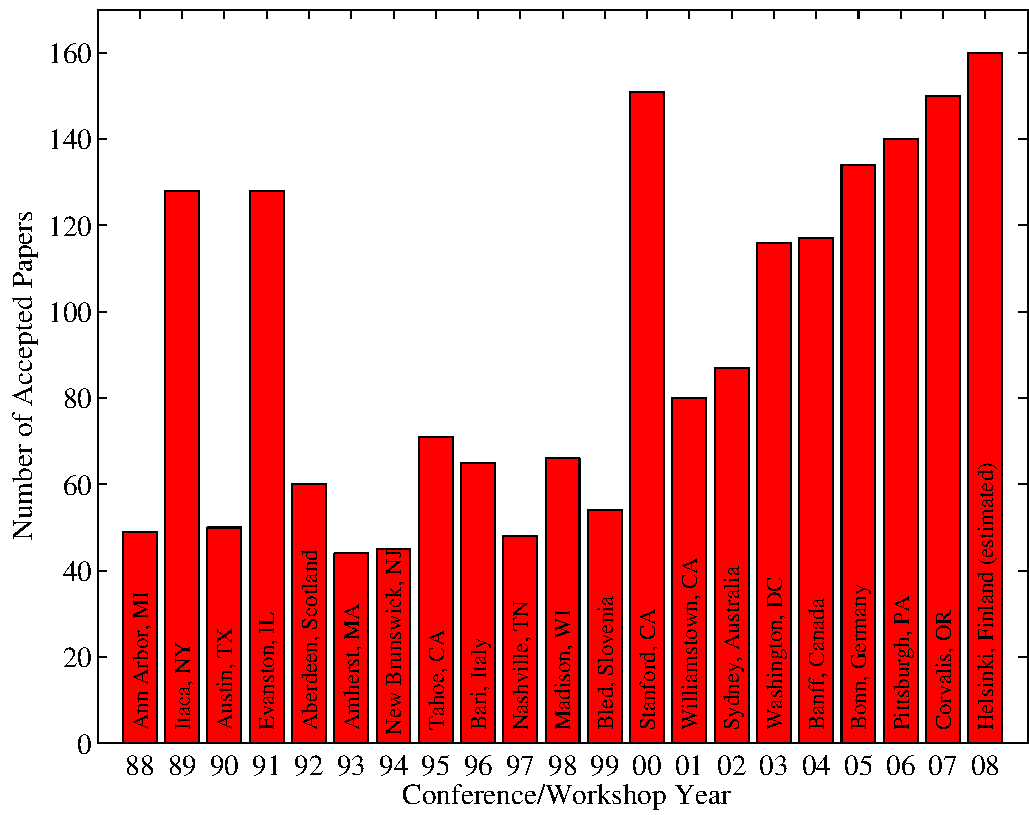
\includegraphics[width=\columnwidth]{icml_numpapers}}
% \caption{Historical locations and number of accepted papers for International
% Machine Learning Conferences (ICML 1993 -- ICML 2008) and International
% Workshops on Machine Learning (ML 1988 -- ML 1992). At the time this figure was
% produced, the number of accepted papers for ICML 2008 was unknown and instead
% estimated.}
% \label{icml-historical}
% \end{center}
% \vskip -0.2in
% \end{figure}

% \subsection{Figures}

% You may want to include figures in the paper to illustrate
% your approach and results. Such artwork should be centered,
% legible, and separated from the text. Lines should be dark and at
% least 0.5~points thick for purposes of reproduction, and text should
% not appear on a gray background.

% Label all distinct components of each figure. If the figure takes the
% form of a graph, then give a name for each axis and include a legend
% that briefly describes each curve. Do not include a title inside the
% figure; instead, the caption should serve this function.

% Number figures sequentially, placing the figure number and caption
% \emph{after} the graphics, with at least 0.1~inches of space before
% the caption and 0.1~inches after it, as in
% \cref{icml-historical}. The figure caption should be set in
% 9~point type and centered unless it runs two or more lines, in which
% case it should be flush left. You may float figures to the top or
% bottom of a column, and you may set wide figures across both columns
% (use the environment \texttt{figure*} in \LaTeX). Always place
% two-column figures at the top or bottom of the page.

% \subsection{Algorithms}

% If you are using \LaTeX, please use the ``algorithm'' and ``algorithmic''
% environments to format pseudocode. These require
% the corresponding stylefiles, algorithm.sty and
% algorithmic.sty, which are supplied with this package.
% \cref{alg:example} shows an example.

% \begin{algorithm}[tb]
%   \caption{Bubble Sort}
%   \label{alg:example}
% \begin{algorithmic}
%   \STATE {\bfseries Input:} data $x_i$, size $m$
%   \REPEAT
%   \STATE Initialize $noChange = true$.
%   \FOR{$i=1$ {\bfseries to} $m-1$}
%   \IF{$x_i > x_{i+1}$}
%   \STATE Swap $x_i$ and $x_{i+1}$
%   \STATE $noChange = false$
%   \ENDIF
%   \ENDFOR
%   \UNTIL{$noChange$ is $true$}
% \end{algorithmic}
% \end{algorithm}

% \subsection{Tables}

% You may also want to include tables that summarize material. Like
% figures, these should be centered, legible, and numbered consecutively.
% However, place the title \emph{above} the table with at least
% 0.1~inches of space before the title and the same after it, as in
% \cref{sample-table}. The table title should be set in 9~point
% type and centered unless it runs two or more lines, in which case it
% should be flush left.

% % Note use of \abovespace and \belowspace to get reasonable spacing
% % above and below tabular lines.

% \begin{table}[t]
% \caption{Classification accuracies for naive Bayes and flexible
% Bayes on various data sets.}
% \label{sample-table}
% \vskip 0.15in
% \begin{center}
% \begin{small}
% \begin{sc}
% \begin{tabular}{lcccr}
% \toprule
% Data set & Naive & Flexible & Better? \\
% \midrule
% Breast    & 95.9$\pm$ 0.2& 96.7$\pm$ 0.2& $\surd$ \\
% Cleveland & 83.3$\pm$ 0.6& 80.0$\pm$ 0.6& $\times$\\
% Glass2    & 61.9$\pm$ 1.4& 83.8$\pm$ 0.7& $\surd$ \\
% Credit    & 74.8$\pm$ 0.5& 78.3$\pm$ 0.6&         \\
% Horse     & 73.3$\pm$ 0.9& 69.7$\pm$ 1.0& $\times$\\
% Meta      & 67.1$\pm$ 0.6& 76.5$\pm$ 0.5& $\surd$ \\
% Pima      & 75.1$\pm$ 0.6& 73.9$\pm$ 0.5&         \\
% Vehicle   & 44.9$\pm$ 0.6& 61.5$\pm$ 0.4& $\surd$ \\
% \bottomrule
% \end{tabular}
% \end{sc}
% \end{small}
% \end{center}
% \vskip -0.1in
% \end{table}

% Tables contain textual material, whereas figures contain graphical material.
% Specify the contents of each row and column in the table's topmost
% row. Again, you may float tables to a column's top or bottom, and set
% wide tables across both columns. Place two-column tables at the
% top or bottom of the page.

% \subsection{Theorems and such}
% The preferred way is to number definitions, propositions, lemmas, etc. consecutively, within sections, as shown below.
% \begin{definition}
% \label{def:inj}
% A function $f:X \to Y$ is injective if for any $x,y\in X$ different, $f(x)\ne f(y)$.
% \end{definition}
% Using \cref{def:inj} we immediate get the following result:
% \begin{proposition}
% If $f$ is injective mapping a set $X$ to another set $Y$, 
% the cardinality of $Y$ is at least as large as that of $X$
% \end{proposition}
% \begin{proof} 
% Left as an exercise to the reader. 
% \end{proof}
% \cref{lem:usefullemma} stated next will prove to be useful.
% \begin{lemma}
% \label{lem:usefullemma}
% For any $f:X \to Y$ and $g:Y\to Z$ injective functions, $f \circ g$ is injective.
% \end{lemma}
% \begin{theorem}
% \label{thm:bigtheorem}
% If $f:X\to Y$ is bijective, the cardinality of $X$ and $Y$ are the same.
% \end{theorem}
% An easy corollary of \cref{thm:bigtheorem} is the following:
% \begin{corollary}
% If $f:X\to Y$ is bijective, 
% the cardinality of $X$ is at least as large as that of $Y$.
% \end{corollary}
% \begin{assumption}
% The set $X$ is finite.
% \label{ass:xfinite}
% \end{assumption}
% \begin{remark}
% According to some, it is only the finite case (cf. \cref{ass:xfinite}) that is interesting.
% \end{remark}
%restatable

% \subsection{Citations and References}

% Please use APA reference format regardless of your formatter
% or word processor. If you rely on the \LaTeX\/ bibliographic
% facility, use \texttt{natbib.sty} and \texttt{icml2022.bst}
% included in the style-file package to obtain this format.

% Citations within the text should include the authors' last names and
% year. If the authors' names are included in the sentence, place only
% the year in parentheses, for example when referencing Arthur Samuel's
% pioneering work \yrcite{Samuel59}. Otherwise place the entire
% reference in parentheses with the authors and year separated by a
% comma \cite{Samuel59}. List multiple references separated by
% semicolons \cite{kearns89,Samuel59,mitchell80}. Use the `et~al.'
% construct only for citations with three or more authors or after
% listing all authors to a publication in an earlier reference \cite{MachineLearningI}.

% Authors should cite their own work in the third person
% in the initial version of their paper submitted for blind review.
% Please refer to \cref{author info} for detailed instructions on how to
% cite your own papers.

% Use an unnumbered first-level section heading for the references, and use a
% hanging indent style, with the first line of the reference flush against the
% left margin and subsequent lines indented by 10 points. The references at the
% end of this document give examples for journal articles \cite{Samuel59},
% conference publications \cite{langley00}, book chapters \cite{Newell81}, books
% \cite{DudaHart2nd}, edited volumes \cite{MachineLearningI}, technical reports
% \cite{mitchell80}, and dissertations \cite{kearns89}.

% Alphabetize references by the surnames of the first authors, with
% single author entries preceding multiple author entries. Order
% references for the same authors by year of publication, with the
% earliest first. Make sure that each reference includes all relevant
% information (e.g., page numbers).

% Please put some effort into making references complete, presentable, and
% consistent, e.g. use the actual current name of authors.
% If using bibtex, please protect capital letters of names and
% abbreviations in titles, for example, use \{B\}ayesian or \{L\}ipschitz
% in your .bib file.

% \section*{Accessibility}
% Authors are kindly asked to make their submissions as accessible as possible for everyone including people with disabilities and sensory or neurological differences.
% Tips of how to achieve this and what to pay attention to will be provided on the conference website \url{http://icml.cc/}.

% \section*{Software and Data}

% If a paper is accepted, we strongly encourage the publication of software and data with the
% camera-ready version of the paper whenever appropriate. This can be
% done by including a URL in the camera-ready copy. However, \textbf{do not}
% include URLs that reveal your institution or identity in your
% submission for review. Instead, provide an anonymous URL or upload
% the material as ``Supplementary Material'' into the CMT reviewing
% system. Note that reviewers are not required to look at this material
% when writing their review.

% % Acknowledgements should only appear in the accepted version.
% \section*{Acknowledgements}

% \textbf{Do not} include acknowledgements in the initial version of
% the paper submitted for blind review.

% If a paper is accepted, the final camera-ready version can (and
% probably should) include acknowledgements. In this case, please
% place such acknowledgements in an unnumbered section at the
% end of the paper. Typically, this will include thanks to reviewers
% who gave useful comments, to colleagues who contributed to the ideas,
% and to funding agencies and corporate sponsors that provided financial
% support.


% % In the unusual situation where you want a paper to appear in the
% % references without citing it in the main text, use \nocite
% % \nocite{langley00}

% % \bibliography{example_paper}
% % \bibliographystyle{icml2022}


% %%%%%%%%%%%%%%%%%%%%%%%%%%%%%%%%%%%%%%%%%%%%%%%%%%%%%%%%%%%%%%%%%%%%%%%%%%%%%%%
% %%%%%%%%%%%%%%%%%%%%%%%%%%%%%%%%%%%%%%%%%%%%%%%%%%%%%%%%%%%%%%%%%%%%%%%%%%%%%%%
% % APPENDIX
% %%%%%%%%%%%%%%%%%%%%%%%%%%%%%%%%%%%%%%%%%%%%%%%%%%%%%%%%%%%%%%%%%%%%%%%%%%%%%%%
% %%%%%%%%%%%%%%%%%%%%%%%%%%%%%%%%%%%%%%%%%%%%%%%%%%%%%%%%%%%%%%%%%%%%%%%%%%%%%%%
% \newpage
% \appendix
% \onecolumn
% \section{You \emph{can} have an appendix here.}

% You can have as much text here as you want. The main body must be at most $8$ pages long.
% For the final version, one more page can be added.
% If you want, you can use an appendix like this one, even using the one-column format.
% %%%%%%%%%%%%%%%%%%%%%%%%%%%%%%%%%%%%%%%%%%%%%%%%%%%%%%%%%%%%%%%%%%%%%%%%%%%%%%%
% %%%%%%%%%%%%%%%%%%%%%%%%%%%%%%%%%%%%%%%%%%%%%%%%%%%%%%%%%%%%%%%%%%%%%%%%%%%%%%%


\end{document}


% % This document was modified from the file originally made available by
% % Pat Langley and Andrea Danyluk for ICML-2K. This version was created
% % by Iain Murray in 2018, and modified by Alexandre Bouchard in
% % 2019 and 2021 and by Csaba Szepesvari, Gang Niu and Sivan Sabato in 2022. 
% % Previous contributors include Dan Roy, Lise Getoor and Tobias
% % Scheffer, which was slightly modified from the 2010 version by
% % Thorsten Joachims & Johannes Fuernkranz, slightly modified from the
% % 2009 version by Kiri Wagstaff and Sam Roweis's 2008 version, which is
% % slightly modified from Prasad Tadepalli's 2007 version which is a
% % lightly changed version of the previous year's version by Andrew
% % Moore, which was in turn edited from those of Kristian Kersting and
% % Codrina Lauth. Alex Smola contributed to the algorithmic style files.
